\documentclass[12pt,letter]{report}
\usepackage{amsmath,amsthm,amsfonts,amssymb,graphicx,multicol}
\usepackage[mathscr]{euscript}
\usepackage[style=alphabetic]{biblatex}
\usepackage{csquotes}
\usepackage{float}
\usepackage{tikz-cd}
\usetikzlibrary{decorations.pathmorphing, arrows.meta}
\setlength{\marginparwidth}{2cm}
\usepackage{todonotes}
\addbibresource{Referencias.bib}



\usepackage[T1]{fontenc}
\usepackage[spanish]{babel}
\usepackage[left=2.5cm, right=2.5cm, top=2.5cm, bottom=2.5cm]{geometry}
\graphicspath{{./img/}}
%\usepackage{pgfplots}
%\usepackage[hidelinks]{hyperref}
%\hypersetup{
%     colorlinks=true,
%     linkcolor=blue,
%     filecolor=blue,
%     citecolor = red,      
%     urlcolor=cyan,
%     }

\setcounter{MaxMatrixCols}{10}
\newtheorem{theo}{Teorema}[chapter]
\newtheorem{prop}[theo]{Proposici\'on}
\newtheorem{coro}[theo]{Corolario}
\newtheorem{lema}[theo]{Lema}
\theoremstyle{definition}
\newtheorem{definition}[theo]{Definición}
\newtheorem*{obs}{Observación}
\newtheorem{ejp}{Ejemplo}

\newcommand{\comments}[1]{}



\def \A{{\mathcal A}}
\def \B{{\mathcal B}}
\def \C{{\mathcal C}}
\def \D{{\mathcal D}}
\def \F{{\mathcal F}}
\def \E{{\mathcal E}}
\def \H{{\mathcal H}}
\def \I{{\mathcal I}}
\def \L{{\mathcal L}}
\def \K{{\mathbb K}}
\def \N{{\mathbb N}} 
\def \O{{\mathcal O}}
\def \Pa{{\mathbb P}}
\def \P{{\mathcal P}}
\def \pp{\mathfrak p }
\def \Q{{\mathbb Q}}
\def \R{{\mathbb R}}
\def \S{{\mathcal S}}
\def \T{{\mathcal T}}
\def \U{{\mathcal U}}
\def \Z{{\mathbb Z}}


\DeclareMathOperator{\Ob}{Ob}
\DeclareMathOperator{\Hom}{Hom}

\def \id{{\mathrm{id}}}
\def \Mor{{\mathrm{Mor}}}
\def \Top{{\mathrm{Top}}}
\def \Gav{{\mathrm{Gav}}}
\def \Et{{\mathrm{Et}}}
\def \Con{{\mathrm{Con}}}
\def \Fun{{\mathrm{Fun}}}
\def \Frm{{\mathrm{Frm}}}
\def \top{{\mathscr{TOP}}}
\def \op{{\mathrm{op}}}
\def \Vect{{\mathrm{Vect}}}
\def \Grp{{\mathrm{Grp}}}
\def \Ring{{\mathrm{Ring}}}
\def \Pos{{\mathrm{Pos}}}
\def \Lan{{\mathrm{Lan}}}
\def \germ{{\mathrm{germ}}}

\renewcommand\qedsymbol{$\blacksquare$}

\begin{document}
\begin{titlepage}
\begin{center}
      {\Huge{UNIVERSIDAD DE GUADALAJARA}}\\
    \vspace{1 cm}
    {\Large{Centro Universitario de Ciencias Exactas e Ingenierías}}
\end{center}
    \vspace*{\fill} 
    \centering
    {\Huge Curso introductorio a la teoría de topos}\\
    \vspace{0.5cm}
    Impartido por:\\
    \vspace{0.5cm}
    {\large  Dr. Luis Ángel Zaldívar Corichi}\\
    \vspace{0.5cm}
    Elaborado por: \\
    \vspace{.5 cm}
    {\large{Alejandro Aceves, Josué  Maldonado,  Juan Carlos Monter} }
    
    \vspace{0.5cm}
    
    \vspace*{\fill} % Ajuste vertical para centrar
\end{titlepage}
\tableofcontents
\chapter{Preliminares}

\section{Construcciones básicas}
\subsection{Categorías}
\begin{definition}[Categoría]
 Una categoría $\C$ consta de los siguientes datos: 
    \begin{enumerate}
        \item[$\bullet$]  Una clase (no necesarimente un cojunto) de objetos $\Ob(\C)$, y una clase de morfismos $\Mor(\C)$. 
        \item[$\bullet$]  A cada par de objetos $X,Y\in \Ob(\C)$ le  
        corresponde  una clase de morfismos (flechas) de $X$ en $Y$, que se denotará por $\Mor_\C(X,Y)$.
        \item[$\bullet$]  Para cada terna de objetos $X,Y,Z\in\Ob(\C)$ está definida una función llamada composición 
	\begin{eqnarray*}
	\Mor_\C(X,Y)\times \Mor_\C(Y,Z)&\rightarrow & \Mor_\C(X,Z)\\
 	(f,g)&\mapsto& g\circ f.
	\end{eqnarray*}
    \end{enumerate}
Además, estos datos satisfacen las siguientes propiedades
\begin{enumerate}
    \item[$\bullet$] La composición es asociativa, es decir, $h\circ(f\circ g)=(h\circ f)\circ g$.
    \item[$\bullet$]  Para cada objeto $X\in \Ob(\C)$ existe un morfismo $Id_X\in \Mor_\C(X,X)$ tal que $f\circ Id_X=Id_X\circ f.$
\end{enumerate}
\end{definition}
Para cualesquiera $X,Y\in\Ob(C)$, una manera de denotar los morfismos de $X$ en $Y$ es por $\Mor_\C(X,Y)$ tal como se muestra en la definición anterior. Sin embargo, también es común denotarlo por  $\Hom_\C(X,Y)$ o $\C(X,Y)$.\\ A continuación se presentan algunos de los ejemplos clásicos de categorías.
\begin{ejp}
\text{ }
    \begin{enumerate}
        \item $\Con$ denota la categoría de conjuntos cuyos objetos son conjuntos y, tiene como morfismos las funciones entre conjuntos. La composición entre morfismos está bien definida, y el morfismo identidad es la función identidad. 
        \item $\Vect_k$ es la categoría que tiene por objetos espacios vectoriales sobre un campo $k$ y, como morfismos transformaciones lineales entre espacios vectoriales.
        \item Sean $A$ y $B$ conjuntos parcialmente ordenados. Un morfismo de $A$ a $B$ es una función monótona (creciente). Esto es, para cualesquiera $a,b\in A$, $a\leq b$ implica que $f(a)\leq f(b)$. Así, los conjuntos parcialmente ordenados junto con sus morfismos constituyen la categoría $\Pos$. Un caso ``más general'' es el siguiente: para cualesquiera dos conjuntos parcialmente ordenados $A$ y $B$, estos se pueden ver como categorías, por lo que un morfismo de $A$ a $B$ no es más que un funtor. 
        \item Algunos ejemplos más son los siguientes: $\Top$ es la categoría de espacios topológicos con morfismos las funciones continuas. Por otro lado, tenemos las categorías de grupos y la categoría de anillos con unidad, $\Grp$ y $\Ring$, cuyos morfismos son homomorfismos de grupos y homomorfismos de anillos, respectivamente. 
    \end{enumerate}
\end{ejp}
\begin{definition}[Categoría pequeña]
    Una categoría $\C$ se dice \emph{pequeña} si la clase objetos $\Ob(\C)$ y la clase de morfismos $\Mor(\C)$ es un conjunto.  
\end{definition}
\begin{definition}[Objeto final/inicial] Sea $\C$ una categoría. Un objeto $T\in\Ob(\C)$ es \emph{final} si para cualquier otro objeto $X\in \Ob(\C)$ existe un único morfismo $f:X\to T$. Análogamente, un objeto $I\in\Ob(\C)$ se dice \emph{inicial} si para cualquier $X\in\Ob(\C)$ existe un único morfismo $g:I\to X$. 
\end{definition}
\begin{prop}
Los objetos finales/inicales, si existen, son únicos salvo 
isomorfismo único \cite{mac2013categories}.
\end{prop}
\subsection{Principio de dualidad}
De la definición de objeto inicial y final, es común pensar que uno es la parte ``dual'' del otro. En la práctica, es común encontrarse con ciertas propiedades que satisface una categoría, sin embargo, muchas de estas propiedades tienen una noción ``dual'' en el sentido de que también se siguen cumpliendo aún cuando se cambia la dirección de las flechas entre los objetos. Esto motiva a la siguiente definición.
\begin{definition}[Categoría opuesta] Sea $\C$ una categoría. Se define la \emph{categoría opuesta} de $\C$, denotada por $\C^{\op}$, como la categoría cuyos objetos son los mismos que los de $\C$, i.e., $\Ob(\C^{\op})=\Ob(\C)$, pero sus morfismos van en sentido opuesto, esto es, si $X^{\op}=X,Y=Y^{\op}\in\C^{\op}$, una flecha $f^{\op}:X^{\op}\rightarrow Y^{\op}$ en $\C^{\op}$ es una flecha $f:Y\rightarrow X$  en $\C$. De este modo se tiene que   
    \[\Mor_{\C^{\op}}(X,Y)=\Mor_\C(Y,X).\]
\end{definition}
Además, la ley de composición está dada por $f^*\circ g^*=(g\circ f)^*$. Observemos  que  $(\C^{\op})^{\op}=\C$, es decir,  la categoría opuesta de $\C^{\op}$ es la categor\'ia original.\\
La importancia de trabajar con la categoría dual reside en el siguiente resultado conocido como el principio de dualidad. 
\begin{theo}
    Supongamos la validez, en toda categoría, de un enunciado que expresa la existencia de algún objeto o morfismo o la igualdad de algunas composiciones. Entonces, el \textquotedbl enunciado dual \textquotedbl, que se obtiene al voltear la dirección de las flechas y al sustituir cada composición $f\circ g$ por $g\circ f$ en el enunciado original, es también válido en  toda categoría.
\end{theo}
\subsection{Funtores}
\begin{definition}[Funtor covariante]
Sean $\A$ y $\B$ categorías. Un funtor \emph{covariante} $F:\A\rightarrow\B$ consiste de lo siguiente:
\begin{enumerate}
\item[$\bullet$] Una asignación en objetos: $F:\Ob(\A)\rightarrow \Ob(\B)$.
\item[$\bullet$] Para cada $X,Y\in\Ob(\A)$ se tiene una asignación
\[F: \mathrm{Mor}_\mathcal{A}(X,Y)\rightarrow \mathrm{Mor}_\mathcal{B}(F(X),F(Y)).\]	
\end{enumerate}
Que satisfacen las siguientes propiedades.
\begin{enumerate}
		\item[$\bullet$] $F$ respeta la identidad:	
		\[ F(Id_X)=Id_{F(X)}. \]
		\item[$\bullet$] Respeta la composición:
		\[ F(g\circ f) = F(g)\circ F(f).\]
\end{enumerate}
\end{definition}
\begin{definition}[Funtor contravariante] Diremos que un funtor es \emph{contravaruiante} si corresponde a un funtor covariante de la forma $F:\A^\op\rightarrow\B$.
\end{definition}
De la definición anterior, se tiene que si $F:\A\to\B$ y $G:\B\to\C$ son funtores, entonces su composición $G\circ F:\A\to\C$ está dada por
 \begin{enumerate}
     \item[i)] El compuesto en objetos, 
     \[(G_0\circ F_0):A_0\to C_0,\quad A_0\in\A,\text{ } C_0\in\C.\]
     \item[ii)] Para cada $A,B\in\mathcal{C}$, el compuesto en morfismos
     \[(G_{F(A),F(B)}\circ F_{A,B}):\Mor_\A(A,B)\to\Mor_\C(G(F(A)),G(F(B))).\]
 \end{enumerate}
 Con esto en mente, definimos lo siguiente.
\begin{definition}
Sean $\A$ y $\B$ categorías. Diremos que $\A$ y $\B$ son \emph{isomorfas} si existen funtores $F:\A\rightarrow \B$ y $G:\B\rightarrow \A$ tal que uno es inverso del otro, i.e., $F\circ G= \id_\B$ y $G\circ F=\id_\A$.
\end{definition}
\todo{Añadir ejemplos}
	
\subsection{Transformaciones naturales}
La manera de relacionar objetos de una categoría es mediante sus morfismos. Como vimos anteriormente, dadas dos categorías es posible obtener información de una a partir de la otra mediante un funtor. En esta sección, estamos interesados en estudiar transformaciones naturales, que a grandes rasgos, estas se pueden entender como morfismos entre funtores.
\begin{definition}[Transformación natural] Sean $F,G:\A\to\B$ funtores. Un \emph{transformación natural} es una tupla $(F,\eta, G)$, en donde $\eta:F\to G$ es una colección de morfismos $\eta_A:F(A)\to G(A)$ en $\B$ tal que 
\begin{enumerate}
    \item Para cada $A\in\mathcal{A}$, se tiene que $\eta_\mathcal{A}:F(A)\rightarrow G(A)$.
    \item Para toda $f\in\A(A,B)$, el siguiente diagrama 
    \begin{center}
	\par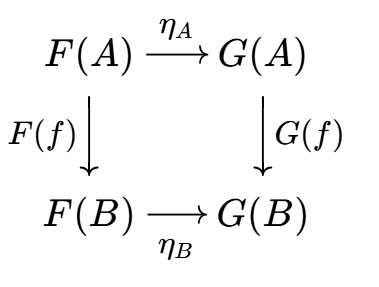
\includegraphics[height=0.22\textwidth]{diagram1.5.1.png}
    \end{center}
    conmuta.
\end{enumerate}
\end{definition}
Si $\eta_A:F(A)\to G(A)$ es un isomorfismo para todo $A\in\Ob(\A)$, diremos que $\eta:F\to G$ es un \emph{isomorfismo natural}, el cual denotamos por $F\cong G$. De esto se sigue que  $\eta^{-1}:F\to G$ dada por $\eta^{-1}_A=(\eta_A)^{-1}$ también es una transformación natural.
\begin{ejp}
Sea $\A$ una categoría pequeña y $\B$ una categoría arbitraria. La categoría de funtores, denotada por $\Fun(\mathcal{A},\mathcal{B})$ (o algunas veces también es denotada por $[\mathcal{A},\mathcal{B}]$), tiene como objetos funtores con dominio $\mathcal{A}$ y codominio $\mathcal{B}$. Para cualesquiera dos funtores en $\Fun(\A,\B)$, un morfismo entre estos es una transformación natural.
 \end{ejp}
 \begin{definition}[Funtor representable] Sea $\C$ una categoría y $F:\C\to\Con$ un funtor. Diremos que $F$ es \emph{representable} si existe un isomorfismo natural entre $F$ y $\Hom(A,-)$, para algún $A\in \Ob(\C)$. En este caso, se dice que $F$ es representado por $A$.
 \end{definition}
Una caracterización de cuando un funtor es representable es la siguiente (veáse \cite{mac2013categories}). Un funtor $F:\C^\op\to\Con$ es representable si, y solo si,  $F\cong h_X$ para algún $X\in\Top$. Esto motiva a enunciar uno  de los resultados de mayor importancia en la teoría de categorías.\todo{Añadir en los ejemplos de funtores el funtor de puntos $h_X$.}
 \begin{lema}[Lema de Yoneda] Sea $F:\C\to\Con$ un funtor. Dado el funtor $\Hom(C,-)$, se tiene que el morfismo
 \begin{eqnarray*}
     \varphi:\Hom(\Hom(A,-))&\to& F(A)\\
     \eta&\mapsto& \eta_A
 \end{eqnarray*}
es un isomorfismo.
 \end{lema}

\section{Límites/colímites}
\subsection{Límites}

\begin{definition}
    Sea $F:\A\to\C$ un funtor. Un \emph{cono} sobre $F$ es una pareja $(C,\langle P_A\rangle_{A\in\A})$ que consiste de lo siguiente:
    \begin{enumerate}
        \item Un objeto $C\in\C$,
        \item Para cada objeto $A\in\A$, se tiene una flecha $(P_A:C\to FA)\in\C$ tal que, para cada flecha $\left(A\xrightarrow{\alpha}A'\right)\in\A$, el siguiente diagrama 
        \begin{figure}[h!]
            \centering
            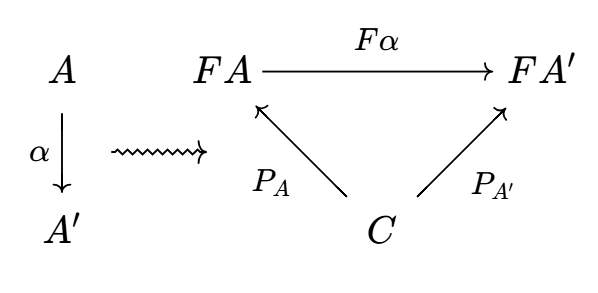
\includegraphics[width=0.35\linewidth]{img/diagrama1.png}
        \end{figure}
        es sólido en $\C$
    \end{enumerate}
\end{definition}
\begin{definition}
    Sea $F:\A\to\C$ un funtor. Un \emph{límite} sobre $F$ es un cono $(L,\langle P_A\rangle_{A\in\A})$ sobre $F$ con la siguiente propiedad: para cualquier otro cono $(M,\langle q_A\rangle_{A\in\A})$ sobre $F$, existe un único morfismo $m:M\to L$ tal que, para todo $A\in \A$, el diagrama
\begin{figure}[H]
    \centering
    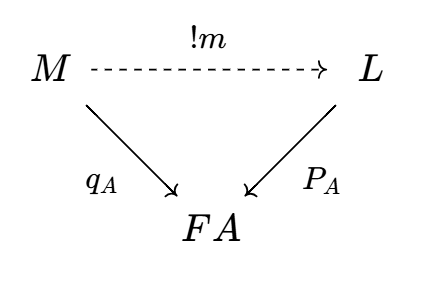
\includegraphics[width=0.3\linewidth]{img/diagrama2.png}
\end{figure}
    conmuta. Esto es, $q_A=P_A\circ m$, para todo $A\in \A$.
\end{definition}
A los morfismos $(P_A:L\to FA,\quad A\in \A)$ se les llama \emph{proyecciones}, y al límite de $F$ se denota como $\varprojlim_{A\in\A} FA$.
\begin{lema}
    El límite de un funtor $F:\A\to\C$, cuando existe, es único salvo isomorfismo natural.
\end{lema}
\begin{proof}
\todo{Pendiente}
\end{proof}
\begin{lema}
    Sea $(L,\langle P_A\rangle_{A\in \A})$ el límite de $F:\A\to\C$. Son morfismos son iguales $\left(
M \overset{f}{\underset{g}{\rightleftarrows}} L \right)\in\C$ si, para todo $A\in \A$, $P_Af=P_Ag$.
\end{lema}
\begin{proof}
    La demostración es inmediata de la propiedad universal del límite. 
\end{proof}

A continuación, se muestran algunos de los ejemplos de límites. 
\begin{ejp}\label{ejp:lim}\text{ }
    \begin{enumerate}
        \item Sea $\A$ una categoría vacía, $\C$ una categoría y $F:\A\to\C$ un funtor. Entonces, el límite de $F$ es un objeto $C\in\Ob(\C)$ tal que, para todo $C'\in\Ob(\C)$, existe un único morfismo $C'\to C$. Es decir, $C$ es el objeto final de $\C$.
        \item Sea $\T$ una categoría con  objetos $\bullet$, $*$, y  $F:\T\to \C$ un funtor. Entonces, un límite para $F$ es 
        \begin{figure}[H]
            \centering
            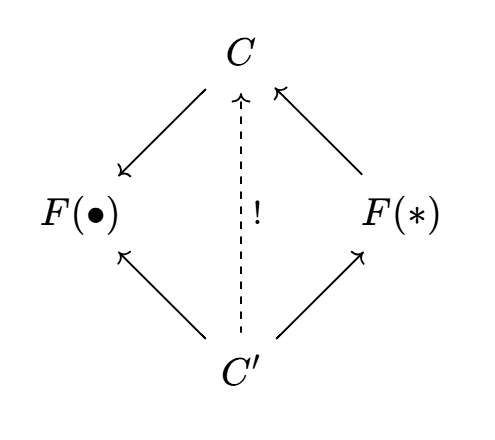
\includegraphics[width=0.3\linewidth]{img/diagrama5.png}
        \end{figure}
        Por lo tanto, $C$ define un producto para $F(\bullet)$ y $F(*)$, el cual denotamos como $C=F(\bullet)\times F(*)$.
        \item Sea $\L$ la categoría que consiste de los objetos $\bullet$ y $*$, dos flechas paralelas de $\bullet$ a $*$, y las respectivas identidades. Sea $F:\L\to\C$ un funtor. De manera diagramática tenemos lo siguiente
        \begin{figure}[H]
            \centering
            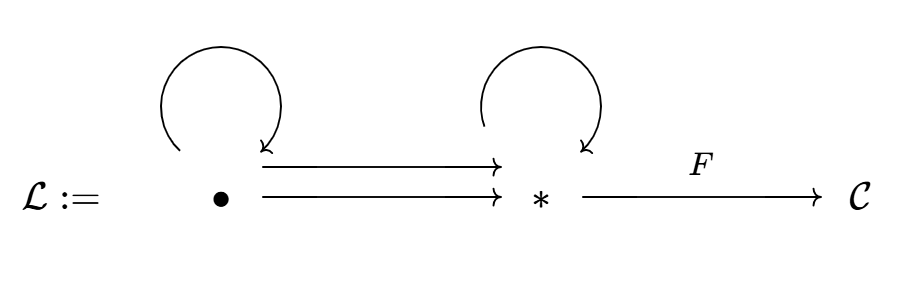
\includegraphics[width=0.5\linewidth]{img/diagrama6.png}
        \end{figure}
        Así, el límite sobre $\F$ de la forma $\L$ es 
        \begin{figure}[H]
            \centering
            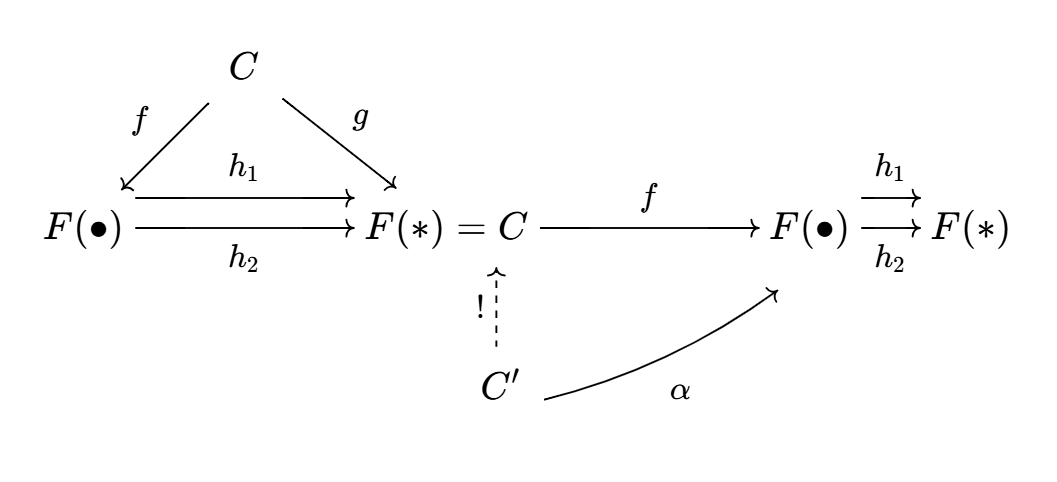
\includegraphics[width=0.6\linewidth]{img/diagrama7.png}
        \end{figure}
        Del diagrama anterior se tiene que, $g=h_1\circ f=h_2\circ f$. Por lo tanto, $C$ es el igualador de $F(\L)$.
        \item Sea $P$ la categoría que consiste de tres objetos $a$, $b$ y $c$, dos flechas $a\to b$, $b\to c$, y las respectivas identidades. Sea $F:P\to\C$ un funtor. En un diagrama se tiene que
        \begin{figure}[H]
            \centering
            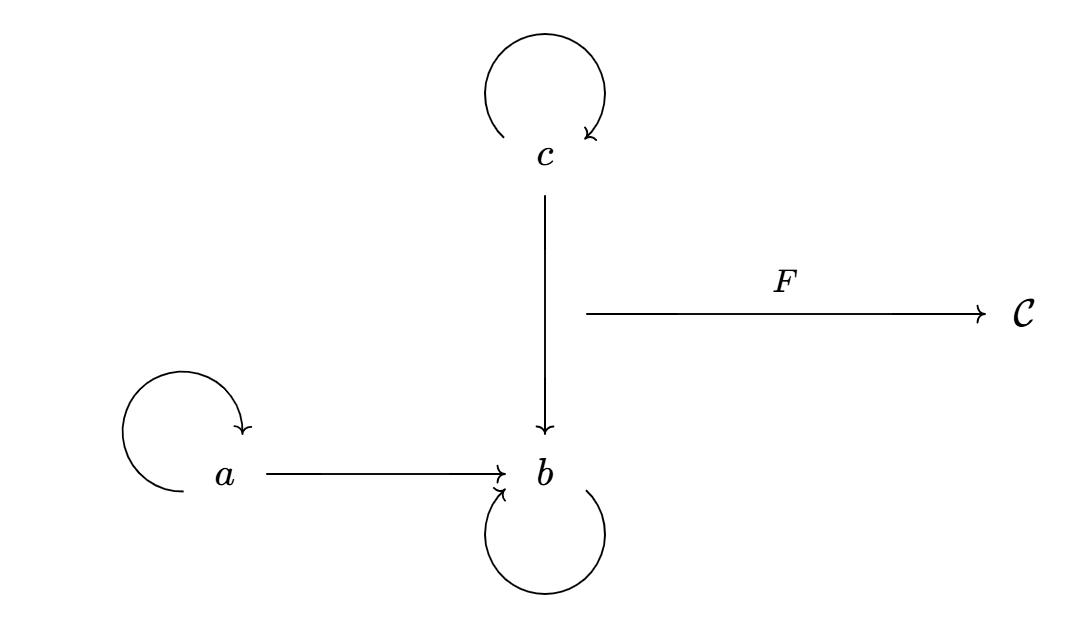
\includegraphics[width=0.6\linewidth]{img/diagrama8.png}
        \end{figure}
       Por lo cual, un límite sobre $F$ de la forma $P$ es el pullback
       \begin{figure}[H]
           \centering
           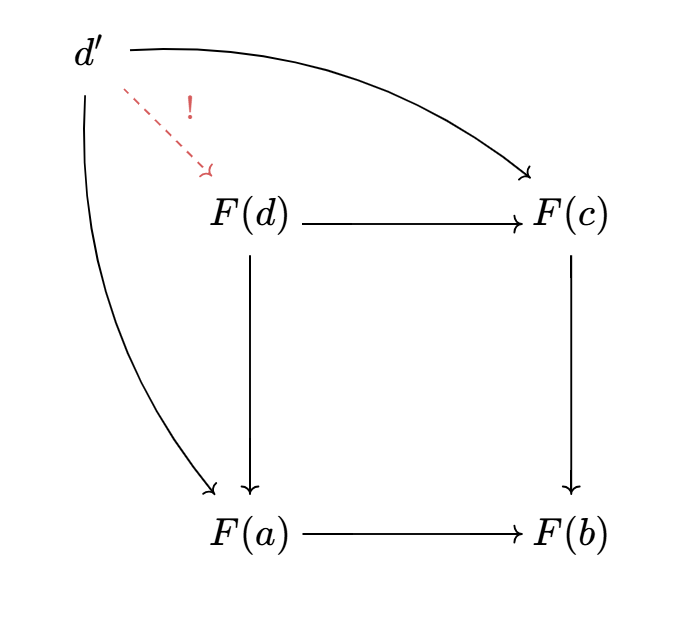
\includegraphics[width=0.38\linewidth]{img/diagrama9.png}
       \end{figure}
    \end{enumerate}
\end{ejp}
\subsection{Colímites}
\begin{definition}
    Sea $F:\A\to\C$ un funtor. Un \emph{cocono} sobre $F$ es una pareja  $(C,\langle s_A\rangle)_{A\in\A}$ que consiste de lo siguiente 
    \begin{enumerate}
        \item Un objeto $C\in \C$.
        \item Para cada $A\in\A$, un morfismo $(s_A:FA\to C)\in\C$ tal que, para cada flecha $\left(A\xrightarrow{\alpha}A'\right)\in\A$, el siguiente diagrama 
        \begin{figure}[h!]
            \centering
            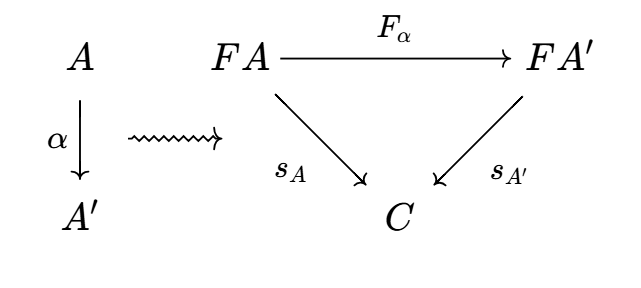
\includegraphics[width=0.4\linewidth]{img/diagrama3.png}
        \end{figure}
        conmuta en $\C$. Es decir, $s_A=s_{A'}\circ F_\alpha$.
    \end{enumerate}
\end{definition}
\begin{definition}
    Un \emph{colímite} sobre $F$ es un  cocono $(L,\langle s_A\rangle_{A\in\A})$ con la siguiente propiedad: para cualquier otro cocono $(M,\langle t_A\rangle_{A\in\A})$ el siguiente diagrama es conmutativo
    \begin{figure}[h!]
        \centering
        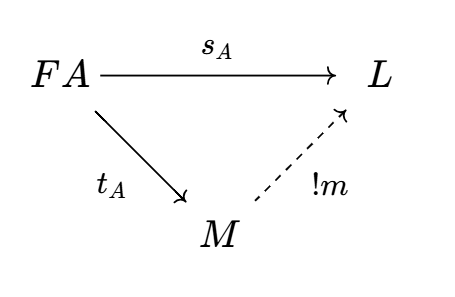
\includegraphics[width=0.3\linewidth]{img/diagrama4.png}
    \end{figure}
    Esto es, para todo $A\in \A$, $t_A=ms_A$.
\end{definition}
Por el principio de dualidad, los ejemplos de colímites se obtienen de manera dual a los ejemplos de límites dados en el Ejemplo \ref{ejp:lim}. 
\begin{lema}\label{lema:igualador}
    Sea $\left( A\xrightarrow{h}B \overset{f}{\underset{g}{\rightrightarrows}} C\right)\in\Con$. Este es un igualador si, y solo si, para cda $b\in B$ tal que $f(b)=g(b)$ implica que existe un único $a\in A$ tal que $h(a)=b$.
\end{lema}
\begin{proof}
    \todo{Pendiente}
\end{proof}
\begin{definition}
    Una categoría $\C$ es \emph{completa} si  cada funtor $F:\D\to\C$  tiene límite, donde $\D$ es una categoría pequeña. Dualmente, $\C$ es \emph{cocompleta} si todo funtor $F:\D\to\C$ tiene colímite. Si $\C$ es completa y cocompleta, diremos que es \emph{bicompleta.}
\end{definition}

\begin{lema}
    La categoría $\Con$ es bicompleta. En particular, los (co)límites de cada funtor se calculan puntualmente.
\end{lema}
\begin{proof}
    \todo{Pendiente}
\end{proof}

\begin{lema}
    Sea $(A,\leq)$ un conjunto parcialmente ordenado. Entonces, la categoría \begin{equation*}
    \Con^{(A,\leq)^{\op}}:[(A,\leq)^{\op},\Con]    
    \end{equation*} 
    es bicompleta y los (co)límites se calculan puntualmente.
\end{lema}
\begin{proof}
    \todo{Pendiente.}
\end{proof}
\begin{definition}
    Sea $\C$ una categoría pequeña.
    \begin{enumerate}
        \item[$\bullet$] Diremos que $\C$ es \emph{finita} si $\Ob(\C)$ y $\Mor(\C)$ son conjuntos finitos.
        \item[$\bullet$] Un límite sobre $F:\C\to \C'$ es \emph{finito} si $\C$ es finita. 
    \end{enumerate}
\end{definition}
\begin{definition}[Categoría filtrante]
    Una categoría $\C$ es \emph{filtrante} si
    \begin{enumerate}
        \item $\C$ es no vacía.
        \item Para cada $C_1, C_2\in \Ob(\C)$ existe $C\in \C$ junto con morfismos $C_1\xrightarrow{f_1} C$ y $C_2\xrightarrow{f_2} C$.
        \item Para cualesquiera $C_1,C_2\in \Ob(\C)$ y morfismos $C_1 \overset{f_1}{\underset{f_2}{\rightrightarrows}} C_2$ existe $C_3\in\Ob(\C)$ y un morfismo $C_1 \overset{f_1}{\underset{f_2}{\rightrightarrows}} C_2\xrightarrow{h} C_3$ tal que $hf_1=hf_2$.
    \end{enumerate}
\end{definition}
\begin{definition}
    Un \emph{colímite} sobre $F:\C\to\D$ es filtrante si $\C$ es filtrante.
\end{definition}
\begin{lema}
    Sea $F:\B\to\C$ un funtor con $\B$ finita y $\C$ filtrante. Entonces, existe un cono sobre $F$ en $\C$.
\end{lema}
La demostración se sigue del siguiente resultado. 
\begin{prop} Sea $\C$ una categoría pequeña.
    \begin{enumerate}
        \item Sea $\{C_i\mid i\in I\}$ un conjunto finito de objetos en $\C$. Entonces, podemos encontrar un objeto $C\in\C$ y morfismos $\{C_i\to C\mid i\in I\}$. 
        \item  Dado un conjunto finito $\{f_i:C\to C'\mid i\in I\}$, podemos encontrar un objeto $C''\in \C$ y un morfismo $C'\xrightarrow{f} C''$ tal que $ff_i=ff_j$, para todo $i,j\in I$. 
    \end{enumerate}
\end{prop}
\begin{proof}
    
\end{proof}
\section{Adjunciones}
\begin{definition}[Adjunción]
Sean $\C$ y $\D$ categorías. Una \emph{adjunción} entre $\C$ y $\D$ es una terna $(F,G,\varphi)$ donde $\D\overset{F}{\underset{G}{\rightleftarrows}}\C$ son funtores y $\varphi$ es una función que asigna a cada par de objetos $C\in\C$ y $D\in\D$ una biyección
\begin{equation*}
\varphi_{\D,\C}:\D(D,GC)\cong\C(FD,C).
\end{equation*}
En este caso, decimos  que $F$ es adjunto izquierdo y $G$ es adjunto derecho, lo cual es denotado por $F\dashv G$. 
\end{definition}
En lo anterior, $\varphi_{\D,\C}$ de hecho es un ismorfismo natural. El siguiente resultado nos dice que las adjunciones se comportan bien bajo composición.
\begin{lema}
    Sean $\D\overset{F}{\underset{G}{\rightleftarrows}}\C\overset{F'}{\underset{G'}{\rightleftarrows}}\B$ funtores. Si $F\dashv G$ y $F'\dashv G'$, entonces $F'\circ F\dashv G\circ G'$.
\end{lema}
\begin{proof}
    Como $F\dashv G$ se tiene que, para cada par de objetos $C\in \C$ y $D\in \D$, hay una biyección 
    \begin{eqnarray}\label{eq:1.7.1}
        \varphi_{\D,\C}:\D(D,GC)\cong\C(FD,C).
    \end{eqnarray}
    Del mismo modo, al ser $F'\dashv G'$, para cada par de objetos $C'\in C$ y $B\in \B$, existe una biyección
    \begin{equation}\label{eq:1.7.2}
        \varphi_{\C,\B}:\C(C, G'B)\cong\B(F'C', B).
    \end{equation}
    Si $D\in \D$ y $B\in \B$, al primero evaluar en (\ref{eq:1.7.1}) en los objetos $C$ y $G'B\in \C$, y después evaluar (\ref{eq:1.7.2}) en $FC\in\D$ y $B\in \B$, obtenemos
    \begin{eqnarray*}
        \D(D,G(G'B))\cong \C(FD,G'B)\cong\B(F'(FC),B).
    \end{eqnarray*}
    Por lo tanto, $F'\circ F\dashv G\circ G'$ tal como se quería.
\end{proof}
A continuación se enuncian un par de resultados en los que se muestra la relación entre objetos iniciales/finales y adjuntos. Esto es, si una categoría tiene objeto inicial, este da lugar a un adjunto izquierdo. Dualmente, si la categoría tiene objeto  final, este determina un adjunto derecho.
\begin{prop}
    Si $\A$ y $\B$ son categorías con objeto inicial entonces el funtor 
    \begin{eqnarray*}
    \sigma_\A:\A&\to&\A\times \B\\
    A&\mapsto& (A,0)\\
    f&\mapsto& (f,1_0)
  \end{eqnarray*}
  es adjunto izquierdo de la proyección $\pi_\A:\A\times\B\to\A$.
\end{prop}
\begin{prop}
    Sean $\A$, $\B$ y $\C$ categorías con coproductos finitos y funtores 
    \begin{figure}[H]
        \centering
        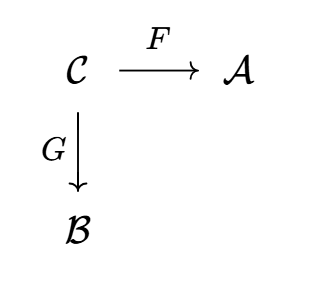
\includegraphics[width=0.18\linewidth]{img/diagram1.4.1.png}
    \end{figure}
    Entonces, el funtor $\langle F,G\rangle:\C\to\A\times\B$ si, y solo si, ambos funtores $F$ y $G$ tienen adjunto izquierdo.
\end{prop}
Ahora, considereos $\C$ y $\D$ dos categorías y $\D\overset{F}{\underset{G}{\rightleftarrows}}\C$ funtores. Si $\left(D\xrightarrow{h}D'\right)\in\D$ y $\left(C\xrightarrow{k}C'\right)\in \D$, de la definición de adjunción, se tienen los siguientes diagramas conmutativos.
    \begin{figure}[H]
        \centering
        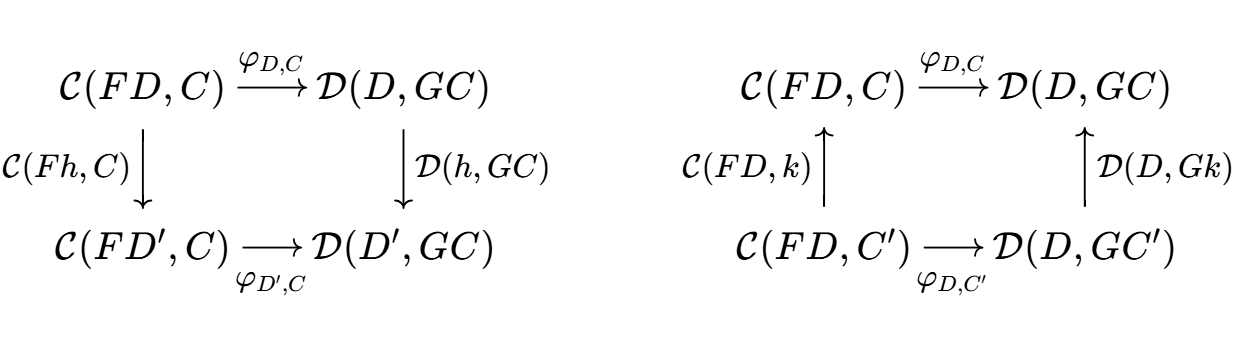
\includegraphics[width=0.8\linewidth]{img/diagram1.4.2.png}
    \end{figure}
    En otras palabras, para todo $FD\xrightarrow{f}C$ se tiene que $\varphi(f\circ Fh)=\varphi(f)h$ y $\varphi(k\circ f)=Gk\circ\varphi f$. Esto es equivalentea que $\varphi^{-1}$ sea también un isomorfismo natural. Es decir, con las mismas flechas y $D'\xrightarrow{g} GC$, se tiene que $\varphi^{-1}(gh)=\varphi^{-1}gFh$ y $\varphi^{-1}(Gkg)=k\varphi^{-1}(g)$. \\
    Tomando el caso particular $C=FD$, se tiene el diagrama conmutativo.
        \begin{figure}[H]
        \centering
        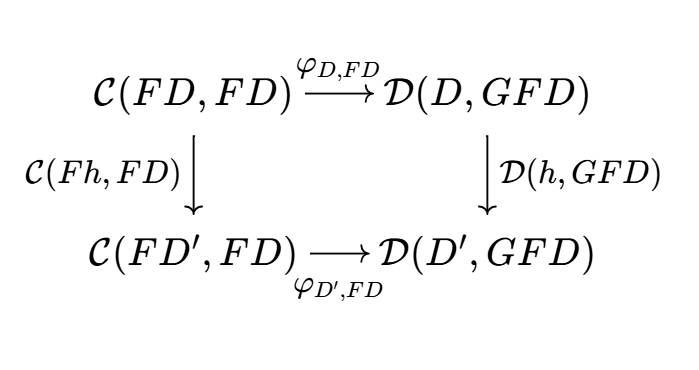
\includegraphics[width=0.45\linewidth]{img/diagram1.4.3.png}
    \end{figure}
    \text{}\\
    Defina $\eta_D=\varphi(1_{FD}):D\to GFD$, para toda $D\in \D$.\\
    \emph{Afirmación. } $\langle \eta_D\mid D\in\D\rangle$ define una transformación natural $\eta:1_D\to GF$. \\
    Basta verificar que el siguiente diagrama conmuta
        \begin{figure}[H]
        \centering
        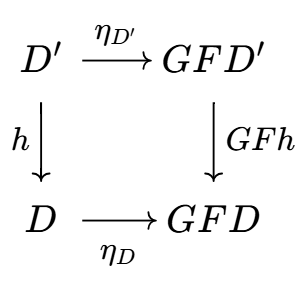
\includegraphics[width=0.2\linewidth]{img/diagram1.4.4.png}
    \end{figure}
    Lo cual es inmediata ya que 
    \begin{equation*}
        GF\varphi(1_D)=\varphi(Fh)=\varphi(1_{D'})h.
    \end{equation*}
    A esta transformación natural $\eta_D:1_D\to GF$ se le llama \emph{unidad de la adjunción} $(F,G,\varphi):\D\to\C$.\\
    Por otro lado, consideremos el caso particular $D=GC$. Entonces se tiene el siguiente diagrama conmutativo. 
           \begin{figure}[H]
        \centering
        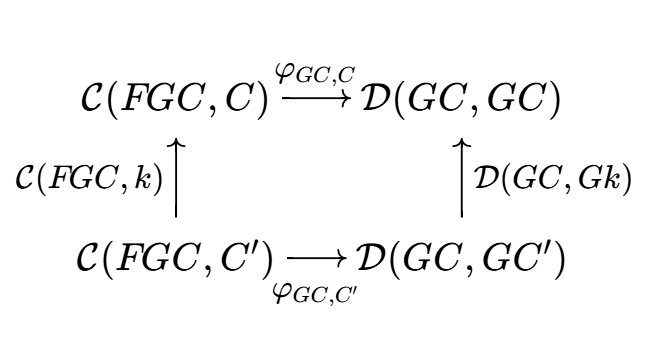
\includegraphics[width=0.45\linewidth]{img/diagram1.4.5.png}
    \end{figure}
    Se define $\varepsilon_C$ como $\phi^{-1}(1_{GA}):FGC\to C$, para toda $C\in \C$. De manera similar a como se hizo con $\eta_D$, se puede verificar que $\epsilon_C$ es una transformación natural, a la cual le llamamos \emph{counidad de la adjunción} $(F,G,\phi): \D\to \C$.
    \begin{definition}[Equivalencia de categorías]
        Dos categorías $\C$ y $\D$ son \emph{equivalentes} si existe una adjunción $(F,G, \eta,\varepsilon):\D\to\C$ tal que la unidad y la counidad son isomorfismos naturales. En este caso, decimos que los funtores $F$ y $G$ son una equivalencia de categorías. 
    \end{definition}
    Para finalizar, veremos una ``aplicación'' de los conceptos vistos en esta sección para el caso particular cuando las categorías son retículas. Dado un conjunto parcialmente ordenado $(A,\leq)$, se dice que es una \emph{retícula} si cada subconjunto finito no vacío $X\subseteq A$ tiene supremo e ínfimo.
    \begin{lema}
    Sean $(A,\leq)$ y $(B,\leq)$ retículas. El funtor $F:\A\to\B$ tiene adjunto derecho si, y solo si, $F$ preserva supremos arbitrarios.     
    \end{lema}
    \begin{proof}\text{}\\
    $\boxed{\Longrightarrow}$
        Supongamos que existe un funtor $G:\B\to \A$ tal que $F\dashv G$. Lo anterior ocurre si, y solo  si, 
        \begin{equation}\label{eq:1.4.1}
            A\leq GB\iff FA\leq B, \quad\forall A\in \Ob(\A), B\in\Ob(\B).
        \end{equation}
        Sea $\bigvee_{i\in I} A_i$ un supremo en $\A$. Esto es, $A\leq \bigvee_{i\in I} A_i$. Dado que $F$ es un funtor, $FA_i\leq F\left(\bigvee_{i\in I}A_i\right)$. Luego, 
        \begin{eqnarray*}
            FA_i\leq \bigvee_{i\in I}FA_i\leq F\left(\bigvee_{i\in I}A_i\right).
        \end{eqnarray*}
        Por (\ref{eq:1.4.1}), se tiene que 
        \begin{eqnarray*}
           A_i\leq G\left(\bigvee_{i\in I}F A_i\right).
        \end{eqnarray*}
        Así, $\bigvee_{i\in I}A_i\leq G\left(\bigvee_{i\in I}FA_i\right)$. Nuevamente, por (\ref{eq:1.4.1}), 
        \begin{eqnarray*}
        F\left(\bigvee_{i\in I}A_i\right)\leq \bigvee_{i\in I}FA_i.
        \end{eqnarray*}
        Ya que se tiene la doble desigualdad, se concluye que $F\left(\bigvee_{i\in I}A_i\right)=\bigvee_{i\in I} FA_i$.\\
        $\boxed{\Longleftarrow}$. Ahora, supongamos que $F$ preserva supremos arbitrarios. Sea $B\in\Ob(\B)$ y tomemos $GB=\bigvee_{FA\leq B}A$. Si $B'\in\Ob(\B)$ es tal que $B'\leq B$, entonces $F(A)\leq B'$ implica que $F(A)\leq B$. Así, 
        \begin{eqnarray*}
            GB'=\bigvee_{FA\leq B'} A\leq\bigvee_{FA\leq B} A=GB
        \end{eqnarray*}
        y $G:\B\to\A$ es funtorial. Ahora, resta probar que $A\leq GB$ si, y solo si $FA\leq B$. Para esto, consideremos $A\in\Ob(\A)$ y $B\in\Ob(\B)$. Si $A\leq GB$, entonces $A\leq\bigvee_{FA\leq B}A$. En virtud de que $F$ preserva supremos arbitrarios, 
        \begin{eqnarray*}
            FA\leq \bigvee_{FA\leq B}FA\leq B.
        \end{eqnarray*}
        Por otro lado, si $FA\leq B$, al ser $G$ un funtor, se tiene que $GFA\leq GB$. Luego, 
        \begin{eqnarray*}
            A=\bigvee_{FA'\leq FA}A'\leq GB
        \end{eqnarray*}
        tal como se quería.
    \end{proof}
\section{Extensiones de Kan}
Recordemos que $\Fun(\A,\B)$ denota la categoría de funtores de la categoría $\A$ en la categoría $\B$, y cuyos morfismos son las transformaciones naturales entre ellos. Lo que se desea probar en esta sección es que la precomposición 
\begin{eqnarray*}
-\circ F:\Fun(\B,\C)&\to&\Fun(\A,\C)\\
G&\mapsto& G\circ F
\end{eqnarray*}
tiene adjunto izquierdo si $\C$ es cocompleta. Como caso particular, esto ocurre si $\C=\Con$.
\begin{definition}[Extensión de Kan]
    Sean $F:\A\to \B$  y $G:\B\to \C$ funtores. La \emph{extensión de Kan izquierdad} de $G$ a lo largo de $F$, si existe, es una pareja $(K:\B\to\C,\text{ }\alpha:G\Rightarrow K\circ F)$, donde $K$ es un funtor y $\alpha$ una transformación natural, que es universal: para cualquier otra pareja $(H:\B\to\C,\text{ }\beta: G\Rightarrow H\circ F )$ existe una única transformación natural $\gamma: K\Rightarrow H$ tal que $(\gamma\circ F)\alpha=\beta$. Es decir, el diagrama 
    \begin{figure}[H]
        \centering
        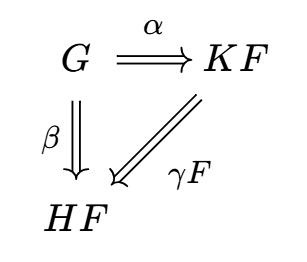
\includegraphics[width=0.2\linewidth]{img/diagram1.4.6.png}
    \end{figure}
    conmuta. El funtor $K$ es denotado por $\Lan_F G$.
\end{definition}
\begin{theo}
    Sean $F:\A\to\B$ y $G:\B\to\C$ funtores. Si $\A$ es pequeña, y $\C$ es cocompleta, entonces la extensión de Kan izquierda de $G$ a lo largo de $F$ existe.
\end{theo}
\begin{proof}
    \todo{Pendiente.}
\end{proof}
Sean $\A$ y $\B$ categorías pequeñas y $\C$ una categoría cocompleta. Consideremos el funtor $-\circ F:\Fun(\B,\C)\to\Fun(\A,\C)$ dado por 
    \begin{figure}[H]
        \centering
        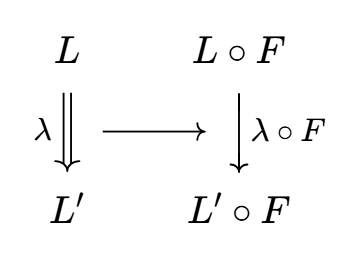
\includegraphics[width=0.25\linewidth]{img/diagram1.4.7.png}
    \end{figure}
Ahora, definimos el funtor $\Lan_{F_{-}}:\Fun(\A,\C)\to\Fun(\B,\C)$
como
    \begin{figure}[H]
        \centering
        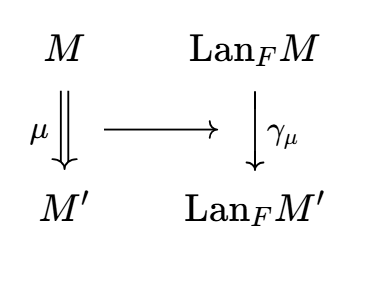
\includegraphics[width=0.25\linewidth]{img/diagram1-4-8.png}
    \end{figure}

donde $\Lan_F M$ es el funtor de la pareja $(\Lan_FM:\B\to\C,\text{ }\alpha_M: M\Rightarrow \Lan_FM\circ F)$. Para culaquier otra pareja $(\Lan_F M':\B\to\C,\text{ }\alpha_{M'}\circ\mu:M\Rightarrow \Lan_F M'\circ F)$, se tiene que $\gamma_\mu:\Lan_F M\Rightarrow \Lan_F M'$ es la única transformación natural tal que $(\gamma_\mu\circ F)\alpha_M=\alpha_{M'}$. Así, se tiene el siguiente resultado. 
\begin{prop}
    Sea $F:\A\to\B$ un funtor y $\C$ una categoría. Si $\A$ es pequeña y $\C$ es cocompleta, entonces $\Lan_{F_{-}}$ es adjunto izquierdo de $-\circ F$.
\end{prop}
\begin{proof}
    \todo{Pendiente.}
\end{proof}
\section{Categorías extensivas}
A lo largo de esta sección, nos referiremos a coproductos finitos como sumas finitas. Para tener una descripción detallada de las demostraciones se sugiere al lector interesado en consultar \cite{Merino2002}.
Dada una categoría $\E$ que admite sumas finitas, y cualesquiera dos objetos $A$ y $B$ de $\E$, se construye la categoría $\E/A\times\E/B $ cuyos objetos son pares $(f,g)$ donde $f:A'\to A$ y $g:B'\to B$, para todo $A', B'\in \Ob(\E)$. Mientras que los morfismos son parejas $(\alpha,\beta)$ donde $\alpha:A'\to A''$ es tal que $f=f'\circ\alpha$, con $f':A''\to A'$ para todo $A', A''$, y lo mismo con $\beta$. A partir de la categoría $\E/A\times\E/B$ se puede construir un funtor que vaya a la categoría $\E/A+B$, esto motiva la siguiente definición.
\begin{definition}
    Sea $\E$ una categoría con sumas finitas y, $A$ y $B$ un par de objetos en $\E$. Se define el funtor 
    \begin{eqnarray*}
        +:\E/A\times\E/B\to\E/A+B
    \end{eqnarray*}
    como aquel que para cada $(f,g)\in\Ob(\E/A\times\E/B)$ le asigna una flecha inducida por la suma. En un diagrama, esto es
    \begin{figure}[H]
        \centering
        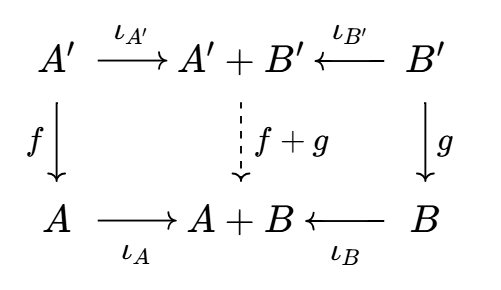
\includegraphics[width=0.35\linewidth]{img/diagrama1.5.1.png}
    \end{figure}
    Mientras que a cada morfismo $(\alpha,\beta)$ en $\E/A\times\E/B$ también le asigna la flecha inducida por la suma tal como lo muestra el siguiente diagrama.
        \begin{figure}[H]
        \centering
        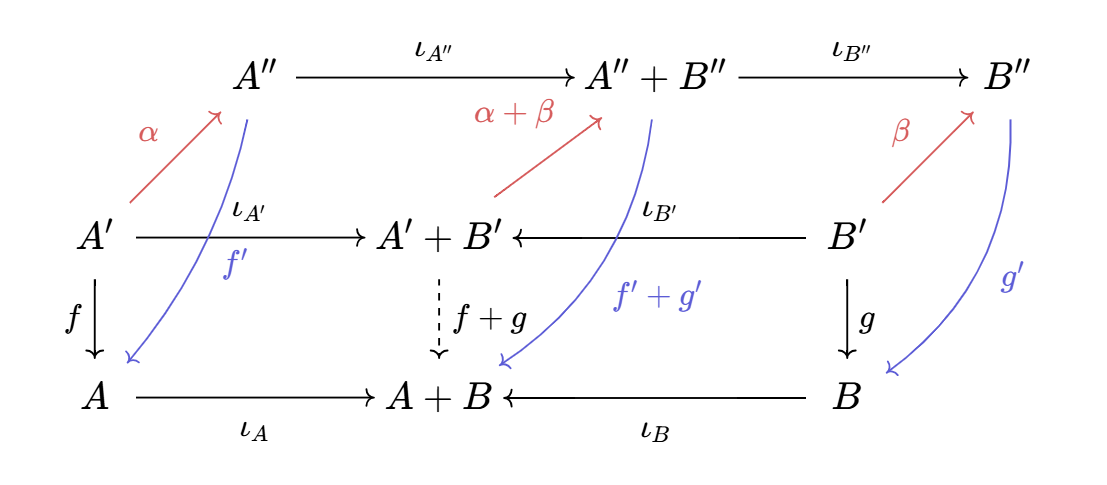
\includegraphics[width=0.75\linewidth]{img/diagram1.5.2.png}
    \end{figure}
\end{definition}
\begin{definition}[Categoría extensiva]
    Sea $\E$ una categoría con sumas finitas. Decimos que $\E$ satisface la \emph{ley extensiva} si, para cada par de objetos $A$ y $B$ de $\E/A\times \E/B$, el funtor $+:\E/A\times\E/B\to\E/A+B$ es una equivalencia de categorías. En este caso, diremos que $\E$ es una categoría extensiva. 
\end{definition}
A grandes rasgos, uno puede pensar en una categoría extensiva como aquella en la que los coproductos (sumas finitas en nuestro caso) se ``comportan bien'' con cierta clase de pullbacks. 
\begin{ejp}
\text{}
    \begin{enumerate}
        \item $\Con$ es extensiva.
        \item $\Top$ es extensiva.
        \item Si $\C$ es una categoría pequeña, entonces la categoría $\mathrm{Fun}[\C^\op,\Con]$ es extensiva.
        \item La categoría de espacios vectoriales sobre un campo $k$, $\Vect_k$, no es extensiva (el coproducto es la suma directa).
    \end{enumerate}
\end{ejp}
\begin{definition}[Sumas universales]
    Dada una categoría $\E$ que admite sumas finitas, diremos que las sumas son \emph{universales} si, para cualquier morfismo $f:S\to A+B$, los productos fibrados a lo largo de las inyecciones existen y el renglón superior del siguiente diagrama
        \begin{figure}[H]
        \centering
        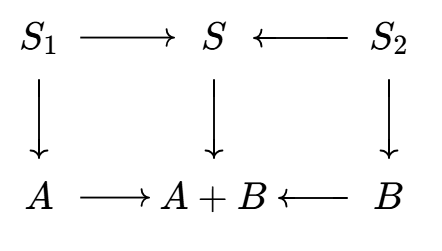
\includegraphics[width=0.3\linewidth]{img/diagrama1.5.3.png}
    \end{figure}
    es una suma. 
\end{definition}
\begin{definition}
    Si una categoría $\E$ tiene objeto inicial $A$, se dice que $A$ es \emph{estricto} si para cada flecha $A\to 0$ se tiene que $A=0$. 
\end{definition}
\begin{lema}
    Si $\E$ es una suma con sumas universales, ebtobces el objeto inicial es estricto.
\end{lema}
\begin{theo}
    Sea $\E$ una categoría con sumas universales. Entonces, $\E$ es extensiva si, y solo si, satisface lo siguiente.
    \begin{enumerate}
        \item[i)] Para cualquier diagrama conmutativo de la forma
        \begin{figure}[H]
        \centering
        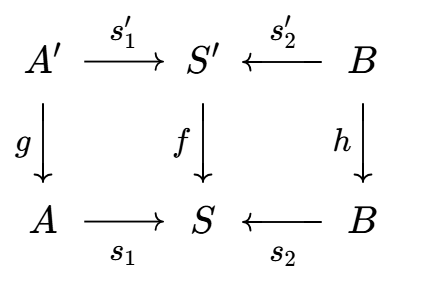
\includegraphics[width=0.3\linewidth]{img/diagrama1.5.4.png}
        \end{figure}
        tal que el renglón inferior es una suma, cumple que el renglón superior también es una suma, entonces ambos cuadrados son productos fibrados.
        \item[ii)] Toda suma en $\E$ es universal.
    \end{enumerate}
\end{theo}
\chapter{Gavillas sobre $\Top$}
Dado un espacio $S$, describir sus propiedades globales puede ser una tarea complicada; en muchas ocasiones, resulta conveniente fijarse en sus propiedades locales, es decir, ver qué ocurre en una vecindad alrededor de un punto $x\in S$, por ejemplo. Así, estudiar propiedades globales de un espacio se convierte en un proceso de pasar de local a global. Intuitivamente, esto refleja algo similar a lo que ocurre con una gavilla en un espacio, ya que esta puede entenderse como una asignación $F$ que a cada abierto $U$ en $S$ se le asigna un conjunto $F(U)$, junto con una noción de ``pegado'' entre los abiertos de $S$. Dependiendo de la naturaleza del problema, en lugar de connjuntos, se pueden considerar grupos, anillos, módulos, etc., esto hace que las gavillas sean una herramienta bastante utilizada  en diversas ramas de la matemática, como topología algebraica, la geometría algebraica y, en general, en álgebra. Precisar el origen de la teoría de gavillas resulta complicado, por lo que muchos consideran un punto de partida y motivación para esta teoría el estudio de la \emph{continuación analítica}, introducida por Riemann para la comprensión de las ``funciones multivaluadas''. Aunque, cabe resaltar que, el desarrollo formal de la teoría de gavillas es gracias a Leray, Serre y Cartan. \\
En esta capítulo se presentan los conceptos fundamentales de la teoría de gavillas en conjuntos, para esto nos basamos en las ideas expuestas en \cite{maclane2012sheaves}.
\section{Gavillas sobre $\Top$}
Dado un espacio $S$, denotamos por $\O(S)$ la categoría cuyos objetos son conjuntos abiertos de $S$. Para cada par de abiertos $U$ y $V$ en $\O(S)$, $\rho:U\to V$ morfismo en $\O(S)$ si, y solo si, $U\subseteq V$.
\begin{definition}[Pregavilla]
    Una \emph{pregavilla} en $\O(S)$ es un funtor $F:\O(S)^\op\to\Con$.
\end{definition}
A un elemento $s\in F(U)$ de la imagen de un abierto $U$ de $S$ se le llama \emph{sección}. Al morfismo $F(\rho):F(V)\to F(U)$ correspondiente a la inclusión $\rho:U\hookrightarrow V$ le llamamos \emph{restricción}. Adoptamos la notación $F(\rho)(s)=s\mid_U=\rho^V_U(s)\in F(U)$ con $s$ una sección de $V$. Con esto en mente, una manera explícita en la que podemos entender una pregavilla es la siguiente: para cada par de abiertos $V\subseteq U$ de $S$ el mapeo restricción actúa como $\rho_V^U: F(U)\to F(V)$ tal que para todo $U\in\O(S)$ se  tiene que $\rho_U^U=\mathrm{id}_U$, y para cualesquiera $W\subseteq V\subseteq U\in\O(S)$ se cumple que, $\rho_W^U=\rho_W^V\circ\rho_V^U$.
\begin{lema}
    Sea $F:\O(S)^\op\to\Con$ un funtor, $U$ un abierto de $S$ y $\{U_i\}_{i\in I}$ una cubierta abierta de $U$. Entonces el diagrama 
    \begin{equation}\label{ec:2.1}
        F(U)\xrightarrow{\varepsilon}\prod_{i\in I} F(U_i)\overset{p}{\underset{q}{\rightrightarrows}}\prod_{i,j\in I}F(U_i\cap U_j),
    \end{equation}
    donde para todo $t\in F(U)$, $e(t)=\langle t\mid_{U_i}\rangle_{i\in I}$ y para toda familia $\langle t_i\in F(U_i)\rangle_{i\in I}$, $p(\langle t_i\rangle_{i\in I})=\langle t_i\mid_{(U_i\cap U_j)}\rangle_{i,j\in I}$, siempre existe y se cumple que $pe=qe$.
\end{lema}
\begin{proof}

\end{proof}
\begin{definition}[Pregavilla separada] Una pregavilla $F:\O(S)^{\op}\to\Con$ se dice \emph{separada} si la función $e$ de (\ref{ec:2.1}) es inyectiva. 
\end{definition}
\begin{definition}[Gavilla]
    Una \emph{gavilla} de conjuntos sobre un espacio topológico $S$ es un funtor $F:\O(S)^\op\to\Con$ tal que para todo conjunto abierto $U$ de $S$ existe una cubierta abierta $\{U_i\}_{i\in I}$ de tal modo que (\ref{ec:2.1}) es un igualador.  
\end{definition}
Es decir, una gavilla es pregavilla separada. En la literatura (veáse \cite{tennison1975sheaf}, por ejemplo) es común definir una gavilla como una pregavilla que satisface lo siguiente.
    \begin{enumerate}
        \item[i).] Sea $U\in\O(S)$. Si $\{U_i\}_{i\in I}$ es una cubierta abierta para $U$ y para cualesquiera dos secciones $s$ y $s'$ tales que $\rho^U_{U_i}(s)=\rho^U_{U_i}(s')$, se tiene que $s=s'$.
        \item[ii).] Sea $U\in\O(S)$ y $\{U_i\}_{i\in I}$ una cubierta de $U$. Si $\{s_i\}_{i\in I}$ es una familia de secciones de $F$, donde $s_i\in F(U_i)$, tal que  $\rho^{U_i}_{U_i\cap U_J}(s_i)=\rho^{U_j}_{U_i\cap U_j}$, para toda $i,j\in I$. entonces existe una sección $s\in F(U)$ tal que $\rho^U_{U_i}(s)=s_i$.
    \end{enumerate}
Obsérvese que la sección $s\in F(U)$ definida en ii), es única por la condición i); a esta condición ii) se le conoce comúnmente como condición de pegado. Resulta que en $\Con$, dar una pregavilla separada es equivalente a dar una pregavilla que satisface i) y ii).
\begin{definition}
    Sea $S$ un espacio topológico. La \emph{categoría de gavillas} sobre $S$ consta de lo siguiente.
    \begin{enumerate}
        \item[$\bullet$] \emph{Objetos}. Gavillas de conjuntos sobre $S$.
        \item[$\bullet$] \emph{Morfismos}. Transformaciones naturales.
    \end{enumerate}
\end{definition}
Algunos ejemplos relvantes de gavillas son los siguientes.
\begin{ejp}
\text{}
    \begin{enumerate}
        \item Sea $U\in\O(S)$. El conjunto 
        \begin{eqnarray*}
            C(U):=\{f:U\to\R\mid f\text{ es continua}\}
        \end{eqnarray*}
        es una gavilla. Para esto, primero veamos que $C(-)$ es funtorial, lo cual demostraría que en efecto es una pregavilla.
        Sea $U\overset{\rho}{\hookrightarrow} V$ con $U,V\in\O(S)$. Entonces, $C(\rho):C(V)\to C(U)$. Tomando la restricción usual, se tiene el siguiente diagrama
        \begin{figure}[H]
            \centering
            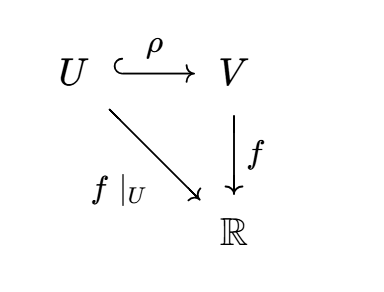
\includegraphics[width=0.25\linewidth]{img/diagram2.1.png}
        \end{figure}
        conmutativo. Esto prueba la funtorialidad, y así $C(-)$ es una pregavilla.\\
        Ahora, veamos que, para cada $U\in \O(S)$Y $\{U_i\}_{i\in I}$ una cubierta abierta para $U$, el siguiente diagrama 
        \begin{eqnarray}\label{ejp2.1}
            C(U)\xrightarrow{e}\prod_{i\in I} C(U_i)\overset{p}{\underset{q}{\rightrightarrows}} \prod_{i,j\in I}C(U_i\cap U_j)
        \end{eqnarray}
        es un igualador en $\Con$. Sea $\{f_i\}_{i\in I}\in\prod_{i\in I}C(U_i)$ tal que $p(\{f_i\})=q(\{f_i\})$. Entonces, $f_i\mid_{U_i\cap U_j}=f_j\mid_{U_i\cap U_j}$ para toda $i,j\in I$. Para cada $U\in\O(S)$, definimos la función $f:U\to\R$ de la siguiente manera
        \begin{equation*}
            f(x)=\begin{cases}
                f_i(x) & \text{si } x\in Ui,\\
                0 &\text{en otro caso.}
            \end{cases}
        \end{equation*}
        Sea $y\in (a,b)\subset\R$ tal que $f(x)=y$, para algún $x\in U$. Ya que $\{U_i\}_{i\in I}$ es una cubierta abierta para $U$, se tiene que $U=\bigcup_{i\in I}U_i$, y en particular $x\in U_i$, para algún $i\in I$. Así, $f_i(x)=f(x)=y$. Luego, como $\{f_i\}\in C(U_i)$ se sigue que $f_i$ es continua para toda $i\in I$; esto implica que existe un abierto $V\subset U_i\subset U$ tal que $x\in V$ y $f_i(V)=f(V)\subset(a,b)$. Por lo tanto, $f\in C(U)$ y $e(f)=\{f_i\}_{i\in I}$. Ahora, supongamos que existe $g\in CU$ tal que $e(g)=\{f_i\}$. Si $x\in U$ entonces, $x\in U_i$ para alguna $i\in I$. De esto se sigue que, $f(x_i)=f(x)=g(x)$. Al tener que $f$ y $g$ tienen el mismo dominio, mismo codominio y misma regla de correspondencia, así $f=g$; lo cual prueba la unicidad de $f$. Por el Lema \ref{lema:igualador}, se sigue que (\ref{ejp2.1}) es un igualador en $\Con$ y $CU$ es una gavilla. 
        \item Sea $U\in \O(S)$. El conjunto
        \begin{eqnarray*}
            C^\infty(U):=\{f:U\to\R\mid f \text{ es suave}\}
        \end{eqnarray*}
        es una gavilla. La demostración de esto es análoga a la del ejemplo anterior.
        \item Sea $U\in\O(S)$. El conjunto de funciones holomorfas
        \begin{eqnarray*}
            \Omega(U):=\{f:U\to\C\mid f\text{ es holomorfa}\}
        \end{eqnarray*}
        es una gavilla. Primero, veamos que $\Omega(-)$ es una pregavilla. Sea $U\overset{\rho}{\hookrightarrow} V$ con $U,V\in\Omega(S)$. Entonces, 
        \begin{eqnarray*}
            \Omega(\rho):\Omega(V)&\to&\Omega(U).
        \end{eqnarray*}
        Por definición, $\Omega(V)=\{f: V\to\C\mid f\text{ es holomorfa}\}$. Tomando la restricción usual, se tiene que el siguiente diagrama conmuta.
        \begin{figure}[H]
            \centering
            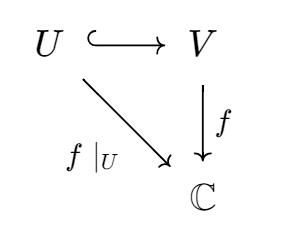
\includegraphics[width=0.2\linewidth]{img/gav3.png}
        \end{figure}
        Así, $\Omega(-)$ es funtorial y, por lo tanto, una pregavilla.\\
        Para probar que $\Omega(-)$ es una gavilla, vamos a verificar las condiciones i) y ii) dadas anteriormente.
        \begin{enumerate}
        \item[i).] Sea $U\in\O(S)$ y $\{U_i\}_{i\in I}$ una cubierta abierta para $U$. Supongamos que $s$ y $s'$ son secciones tales que $\rho^U_{U_i}(s)=\rho^U_{U_i}(s')$. Del siguiente diagrama
            \begin{figure}[H]
            \centering
            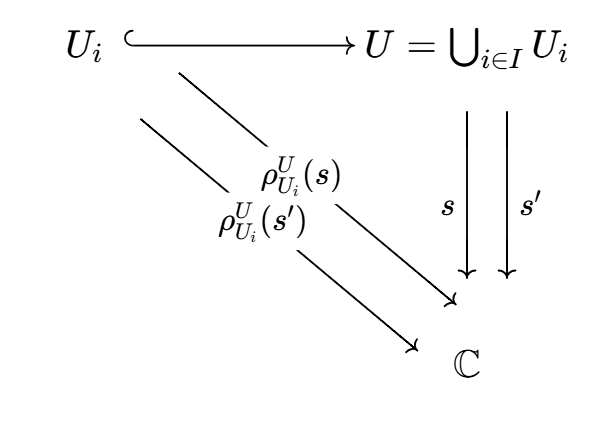
\includegraphics[width=0.4\linewidth]{img/diagram2.2.png}
        \end{figure}
        se tiene que $s=s'$.
        \item[ii).] Supongamos que $f_j:U_j\to\mathbb{C}$ son holomorfas y $f_i\mid_{U_i\cap U_j}=f_j\mid_{U_i\cap U_j}$. En $U=\bigcup_{i\in I}U_i$, definimos $f(w)=f_j(w)$, para toda $w\in U_i$. Para ver que la condición de pegado se satisface, basta verificar que $f$ satisface las condiciones de Cauchy-Riemann. Sea $z=x+iy\in\C$. Entonces, $f(z)=f(x,y)=f(x+iy)=u(x,y)+iv(x,y)$. Luego, 
   
        \begin{eqnarray*}
            \dfrac{\partial f}{\partial z}=\dfrac{\partial u}{\partial x}+i\dfrac{\partial v}{\partial y}&=& \dfrac{\partial u'}{\partial x}+i\dfrac{\partial v'}{\partial y}\quad\text{ con }u'(x,y)+iv'(x,y)=f_j(z)\\
            &=& \dfrac{\partial u'}{\partial x}=-\dfrac{\partial v'}{\partial y} \quad f_j\text{ es holomorfa}\\
            &=& \dfrac{\partial u'}{\partial x}_{u_j}=-\dfrac{\partial v'}{\partial y}_{u_j}
        \end{eqnarray*}
        Por lo tanto, $f_j=f\mid_{U_j}$. Así, $f$ es holomorfa, y $\Omega(-)$ es gavilla.
        \end{enumerate}
\end{enumerate}
\end{ejp}
\section{El funtor $\Gamma$} 
Dado $S$ un espacio topológico, la categoría de rebanadas $\Top/S$ consta de lo siguiente.
\begin{enumerate}
    \item[$\bullet$] \emph{Objetos}. Todas las funciones continuas $f\in\Mor(\Top)$ cuyo codominio son igual a $S$.
    \item[$\bullet$] \emph{Morfismos}. Para cada función continua $f:E\to E'\in\Mor(\Top)$, existen $p:E\to S$ y $p':E'\to S$ tales que $p=p'\circ f$.
    \begin{figure}[H]
        \centering
        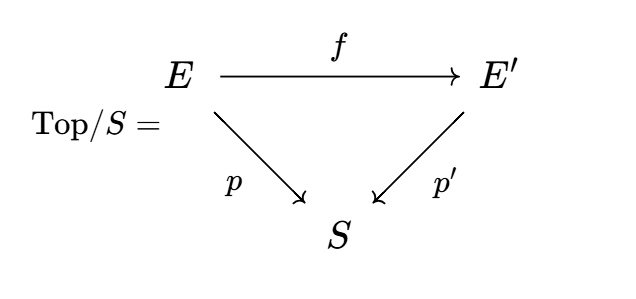
\includegraphics[width=0.42\linewidth]{img/diagram2.2.1.png}
    \end{figure}
\end{enumerate}
A una función continua de la forma $p:E\to S$ le llamamos \emph{haz} sobre $S$, y al espacio $E$ se le conoce como \emph{espacio total}. En topología algebraica es común estudiar un tipo particular de haces, los cuales se llaman haces fibrados, y no deben de confundirse con los haces que estamos estudiando ya que $f$ solo es una función continua y no un homeomorfismo; además, de que no pedimos la condición de localidad trivial como ocurre en el caso de los haces fibrados. \\
Para cada punto $x\in S$, la \emph{fibra asociada} a $x$ es la preimagen  $p^{-1}(x)$. Esto nos permite interpretar al espacio $E$ como un espacio formado por copias de cada fibra parametrizada por los puntos de $S$. Como $p:E\to S$ es una función continua, la preimagen de abiertos manda abiertos en abiertos; por lo cual, para cada $U\in S$ conjunto abierto, se tiene que $p_U:p^{-1}(U)\to U$ es un haz sobre $U$. Más aún, el siguiente diagrama
    \begin{figure}[H]
        \centering
        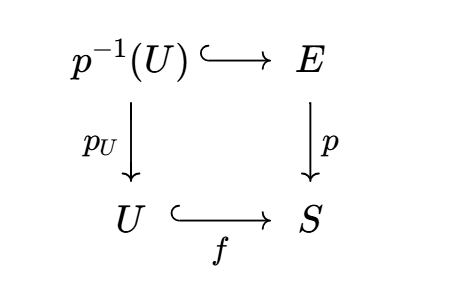
\includegraphics[width=0.32\linewidth]{img/diagram2.2.2.png}
    \end{figure}
\noindent
es un pullback en $\Top$. 
\begin{definition}[Sección] Una \emph{sección} (global) de un haz $p:E\to S$ es una función continua $s:S\to E$ tal que $p\circ s=\id_S$. Una \emph{sección local} de $p$ alrededor de $x\in S$ es una sección de $p_U$. 
\end{definition}
\begin{prop}
    Sea $p:E\to S$ un haz y $f:U\to S$ una función continua. Hay una correspondencia biyectiva entre el conjunto de secciones de $p_U$ y el conjunto de levantamientos de $f$ a $E$, es decir, funciones continuas $h:U\to E$ tal que $ph=f$.
\end{prop}
\begin{proof}
    Por la propiedad universal del pullback, dar una sección de $p_U$ es equivalente a dar un levantamiento $h:U\to E$ de $f$ que hace completar el siguiente diagrama.
        \begin{figure}[H]
        \centering
        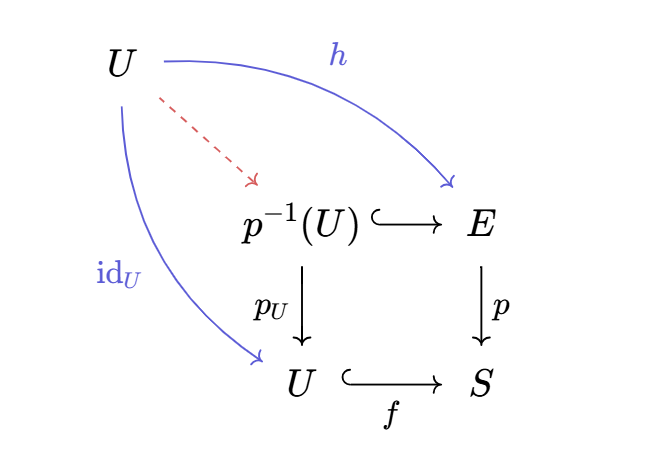
\includegraphics[width=0.43\linewidth]{img/diagram.2.2.3.png}
    \end{figure}
\end{proof}
\noindent
Denotemos por $\Gamma_pU:=\{s\mid s\text{ es una sección local}\}$. Dado un abierto $U$ de $S$ y $V\subset U$, se define
\begin{eqnarray*}
    \Gamma_pU&\to&\Gamma_p V\\
    s&\mapsto& \rho^U_V(s):=s\mid_V.
\end{eqnarray*}
\begin{lema}
    $\Gamma_p:\O(S)^{op}\to\Con$ es un funtor.
\end{lema}

\section{El funtor $\Lambda$}
Sea $P:\O(S)^{\op}\to\Con$ una pregavilla sobre un espacio $S$. Sea $x\in S$ un punto, y consideremos la familia $\O(x):=\{U\in \O(S)\mid x\in U\}$ la familia de vecindades abiertas de $x$ en $S$. Dados $U_\alpha, U_\beta\in \O(x)$ la intersección $U_\gamma:=U_\alpha\cap U_\beta\in\O(x)$ cumple que $U_\gamma\subseteq U_\alpha$ y $U_\gamma\subseteq U_\beta$. Esto es, considerando el orden pacial $\leq$ dado por la contención de abiertos, se tiene que $(\O(x),\leq)$ es un conjunto dirigido. Además, para cada morfismo  $\iota^\beta_\alpha:U_\alpha\hookrightarrow U_\beta$ en $\O(x)$, se tienen morfismos $\phi^\beta_\alpha:= P(\iota^\beta_\alpha): P(U_\beta)\to P(U_\alpha)$ los cuales forman una familia directa en $\Con$, denotada por $(P(\O(x)),\leq)$. \\
Si el colímite de $(P(\O(x)), \leq )$ en $\Con$ existe, este es denotado por $P_x:=\varinjlim P(U_\alpha)$. Para cada familia $\{M_\alpha\}$ indexada por $\O(x)$, este colímite se puede ver de manera explícita como sigue 
\begin{equation*}
     \varinjlim M_\alpha:=\left(\bigsqcup M_\alpha\right)/\sim
\end{equation*}
donde $s\sim t$ ($s\in PU$ y $t\in PV$) si, y solo si, existe un abierto $W$ tal que $W\subseteq U\cap V$ y  $s\mid_W=t\mid_W\in PW$ para $x\in W$. Además, se tienen morfismos canónicos 
\begin{eqnarray*}
    \phi:P(U_\alpha)\to\bigsqcup P(U_\alpha)\to\varinjlim P(U_\alpha).
\end{eqnarray*}
\begin{definition}[Germen]
    Dada una sección $s\in P(U)$, se define su \emph{germen} en el punto $x\in S$, denotado por $[s]_x$, como la imagen  $\phi(s)\in P_x$. 
\end{definition}
Notemos que, para un punto $x\in S$, los elementos de $P_x$ son precisamente las secciones en el punto $x$. A $P_x=\{[s]_x\mid s\in PU, x\in U\in\O(x)\}$ se le conoce como el \emph{tallo} de $P$ en $x$. 
\begin{lema}
    La relación ``$\sim$'' es de equivalencia. 
\end{lema}
\begin{proof}
\text{}
\begin{enumerate}
  \item[$\bullet$]  \emph{Reflexividad.} Sea $U\in\O(S)$ y $s\in PU$. Para $x\in U$, tenemos que $U\subseteq U$ y $s=s\mid_U$. Por lo tanto, $s\sim s$.
   \item[$\bullet$] \emph{Simetría.} Para $U,V\in\O(S)$, sean $s\in PU$ y $t\in PV$ tales que $s\sim t$. Entonces, se cumple la definición y dado que existe $W\subseteq U\cap V$, se sigue que también se cumple $t\sim s$.
    \item[$\bullet$]\emph{Transitividad.} Consideremos $U,V,W\in\O(S)$ y, $s\in PU$, $t\in PV$ y $r\in PW$ tales que $s\sim t$ y $t\sim r$. Entonces, existen $Y\subseteq U\cap V$ y $Y'\subseteq V\cap W$ vecindades de $x$ donde $s\mid_Y=t\mid_{Y}$ y $t\mid_{Y'}=r\mid_{Y'}$. Nótese que $Y\cap Y'$ es una vecindad de $x\in U\cap W$. Como $s\mid_Y=t\mid_Y$ implica que $s\mid_{Y\cap Y'}=t\mid_{Y\cap Y'}$. Además, $t\mid_{Y\cap Y'}=r\mid_{Y\cap Y'}$. Por lo tanto, $s\mid_{Y\cap Y'}=r\mid_{Y \cap Y'}$ y $s\sim r$.
    \end{enumerate}
    Ya que $\sim$ es reflexiva, simétrica y transitiva se tiene que es de equivalencia.
\end{proof}

\begin{lema}
    Sea $P^x:\O(x)\to\Con$. Las funciones $\{\germ_x: P(U)\to\O(x)\}$ tales que para cada sección $s\in P(U)$, $\germ_xs=[s]_x$, forman un cocono colímite sobre $\O(x)$. Más aún, este es filtrante.
\end{lema}
\begin{proof}
    Sean $U,V\in\O(x)$. Entonces, se tiene el siguiente diagrama
    \begin{figure}[H]
        \centering
        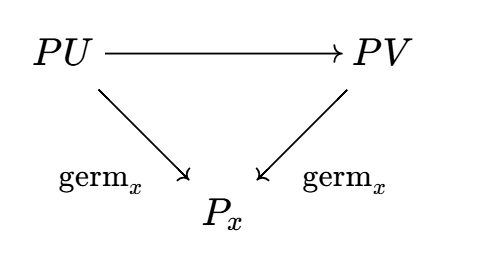
\includegraphics[width=0.3\linewidth]{img/diagram_2.3.1.png}
    \end{figure}
    Si $s\in PU$ es tal que $s\mid_V=PV$, entonces $[s]_x=[s\mid_V]_x$. Por lo tanto, el diagrama anterior conmuta y $(\germ_x:PU\to P_x)_{U\in \O(x)}$ es un cócono. Ahora, consideremos $(\tau_u: PU\to L)_{U\in\O(x)}$ otro cocono sobre $P^{(x)}$. Veamos que existe una única función $t:P_x\to L$ tal que $t\circ\germ_x=\tau$. Esto es, 
    \begin{figure}[H]
        \centering
        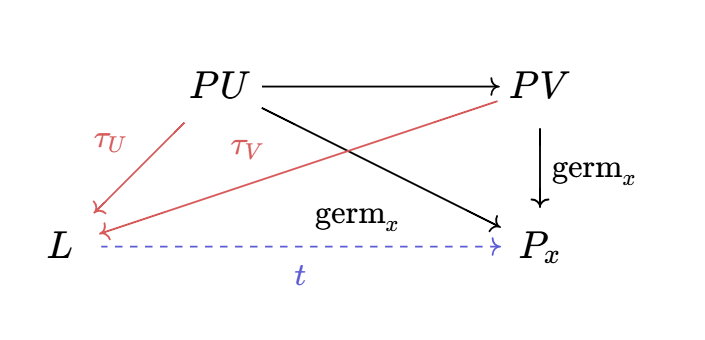
\includegraphics[width=0.45\linewidth]{img/diagram2.3.2.png}
    \end{figure}
    Definamos $t:P_x\to L$ como $t([s]_x)=\tau_U(s)$. Ahora, tomemos $r$ otro representante, i.e., $[s]_x=[r]_x$ implica que existe $W\in U\cap V$ tal que $s\mid_W=r\mid_W$ y $\tau_W(s\mid_W)=\tau_W(r\mid_W)$. Como $\tau$ es un cócono, entonces 
    \begin{eqnarray*}
    \tau_U(s)=\tau_W(s\mid_W)=\tau_W(r\mid_W)=\tau_V(r).
    \end{eqnarray*}
    Por lo tanto, $t$ está bien definida. Ahora, sea $s\in PU$. Entonces, $t\circ\germ_x(s)=t([s]_x)=\tau_U(s)$. Por otro lado, consideremos $l:P_x\to L$ tal que $l\circ\germ_x(s)=\tau$. Si $[s]_x\in P_x$, se tiene que
    \begin{eqnarray*}
        t([s]_x)&=& t\circ\germ_x(s)=\tau(s)\\
        &=& l\circ\germ_x(s)=l([s]_x).
    \end{eqnarray*}
    Por lo tanto, $t$ es única y $\{\germ_x:PU\to P_x\}$ es un cócono límite.
\end{proof}
\begin{lema}
    Cualquier morfismo $h:P\to Q$ de pregavillas (cualquier transformación natural), en cada punto $s\in S$, induce una única función $h_x:P_x\to Q_w$ tal que el diagrama 
    \begin{figure}[H]
        \centering
        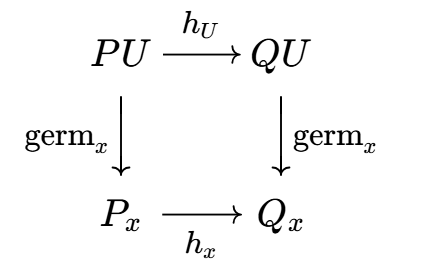
\includegraphics[width=0.3\linewidth]{img/diagram2.3.3.png}
    \end{figure}
    conmuta para cualquier $U\in\O(x)$.
\end{lema}
\begin{proof}
    Sea $h:P\to Q$ una transformación natural. Sean $U,V\in\O(x)$ tal que $V\leq U$. Si $s\in PU$, al ser $h$ natural se tiene que $\germ_x\circ h_V(s\mid_V)=\germ_x(h_V(s)\mid_V)$. Por el lema anterior, $\{\germ_x:PU\to PV\}$ es un cócono límite; así, existe una única función $h_x:P_x\to Q_x$ que hace conmutar el diagrama deseado. Además, $h_x([s]_x)=[h_U(s)]_x$. 
\end{proof}
\noindent
Del resultado anterior, tenemos el diagrama conmutativo
    \begin{figure}[H]
        \centering
        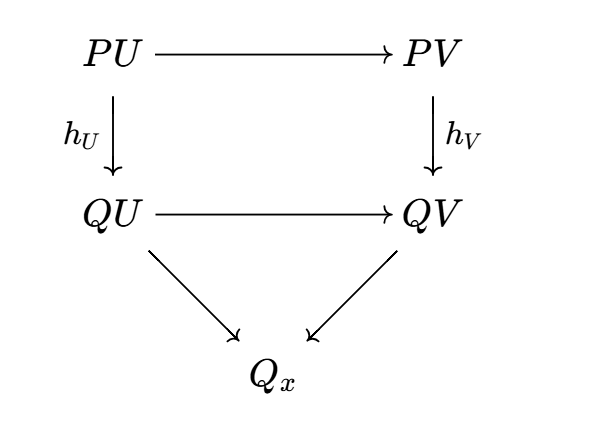
\includegraphics[width=0.37\linewidth]{img/diagram2.3.4.png}
    \end{figure}
\noindent
Un resultado inmediato es el siguiente.
\begin{lema}
    La transformación natural dada por $h\to h_x$ es un funtor de $\Con^{\O(x)^{op}}\to \Con$. Dicho funtor es ``tomar germen en $x$''.
\end{lema}

\begin{proof}
Ya hemos probado que la asignación de objetos y flechas está bien definida. Resta verificar que 
preserva identidades y composiciones.
\begin{itemize}
\item Sea $\id_p\colon P\to P$ en $\Con^{\O(x)^{op}}$, Veamos que $(\id_p)_x=\id_{p_x}$. Sea $[s]_x\in P_x$, por el lema anterior,
cualquier morfismo $\id_p\colon P\to P$ induce $\id_{p_x}$. Así,
\[
\id_{p_x}([s]_x)=[\id_p(s)]_x=[s]_x.
\]
\item Sean $h\colon P\to Q$ y $g\colon Q\to R$ morfismos en $\Con^{\O(x)^{op}}$. Veamos que $(g\circ h)_x=g_x\circ h_x$. Sea $[s]_x\in P_x$ y al ser $h$, $g$ 
\item transformaciones naturales, se tiene que
\[
(g\circ h)_x([s]_x)=g_x([h_U(s)]_x)=[g_U(h_U(s))]_x=g_x\circ h_x([s]_x).
\]
\end{itemize}
\end{proof}

Sea 
\begin{eqnarray*}
\Lambda_p=\bigsqcup_{x\in S}P_x=\bigsqcup_{x\in S}\{[s]_x\mid s\in PU\}
\end{eqnarray*} 
la unión disjunta de germenes sobre $x\in S$. Para toda sección $s\in PU$, definamos las siguientes funciones
\begin{eqnarray*}
    p:\Lambda_p&\to& S\\
    \left[s\right]_x&\mapsto& x,\\
    \hat{s}:U&\to&\Lambda_p\\
    x&\mapsto& \left[s\right]_x.
\end{eqnarray*}
\begin{lema}
    El conjunto $B_p:=\{\hat{s}(U)\mid s\in PU, U\in\O(S)\}$ es una base para una topología en $\Lambda_p$.
\end{lema}

\begin{proof}
    Primero veamos que $\bigcup B_p=\Lambda_p$.
    \begin{itemize}
        \item Se cumple que $\bigcup B_p\subseteq \Lambda_p$, para la otra condición consideremos $[s]_x\in \Lambda_p$, entonces $[s]_x=\hat{s}(U)$ para algún $U\in\O(S)$ y $s\in PU$. Por lo tanto, $[s]_x\in B_p$.
        \item Sean $\hat{s}(U)$, $\hat{r}(V)\in B_p$ y supongamos que $\hat{s}(x)=\hat{r}(y)$, entonces $[s]_x=[r]_y$. Por lo tanto $x=y$ y así existe $W\subset U\cap V$ tal que $s\mid_W=r\mid_W$. Luego $\widehat{s\mid_W}(W)$ es un elemento en $B_p$ tal que
        \[
        [s]_x\in\widehat{s\mid_W}(W)\subset \hat{s}(U)\cap \hat{r}(W).        
        \]
    \end{itemize}
\end{proof}

\begin{obs}
Sean $U,V\in \O(S)$ tales que $V\subset U$ y $s\in PU$. Entonces $\hat{s}(V)=\widehat{s\mid_V}(V)$ para todo $s\in PU$.
\end{obs}

\begin{lema}
Sea $\Lambda_p$ dotado con la topología $B_p$. Entonces $p$ y $\hat{s}$ son continuas. Más aún, $p$ es un haz sobre $S$ y $\hat{s}$ es una sección local de $p$.
\end{lema}

\begin{proof}
\begin{itemize}
\item Sea $V\subseteq S$ abierto y sea $[s]_x\in \Lambda_p$ tal que $[s]_x\in p^{-1}(V)$, entonces $x\in U\cap V$. Consideremos $\widehat{s\mid_{U\cap V}}(U\cap V)\in B_p$. Por la observación 
anterior 
\[
[s]_x=[s\mid_{U\cap V}]_x\in \widehat{s\mid_{U\cap V}}(U\cap V)\subseteq p^{-1}(V).
\]
Por lo tanto, $p$ es continua.

\item Para $\hat{s}\colon U\to \Lambda_p$ sea $\hat{r}(V)\in B_p$ un abierto básico y $x\in U$ tal que $\hat{s}(x)\in \hat{r}(V)$. Entonces $[r]_y=[s]_x$ y $x=y$, de aquí que existe $W\subset U\cap V$ tal que 
$s\mid_W=r\mid_W$. Por lo tanto, $\hat{s}(W)$ es un abierto básico tal que 
\[
[s]_x\in \hat{s}(W)\subseteq \hat{r}(V).
\]
De esta manera se concluye que $\hat{s}$ es continua.
\end{itemize}
Para ver que $\hat{s}$ es una sección local de $p$, basta notar que para todo $x\in U$ se tiene que $p\circ \hat{s}(x)=p([s]_x)=x$, por lo tanto 
$p\circ \hat{s}=\id_U$, es decir, el diagrama
\[\begin{tikzcd}
	U && {\Lambda_p} \\
	& S
	\arrow["{\hat{s}}", from=1-1, to=1-3]
	\arrow["i"', hook, from=1-1, to=2-2]
	\arrow["p", from=1-3, to=2-2]
\end{tikzcd}\]
conmuta.
\end{proof}

\begin{definition}
Sea $f\in \Top$, decimos que $f$ es un \emph{homeomorfismo} si tiene una inversa continua.
\end{definition}

\begin{lema}
    $\hat{s}\colon U\to \hat{s}(U)$ es un homeomorfismo.
\end{lema}

\begin{proof}
Consideremos $V\subset U$ abierto de $S$, entonces $\hat{s}(V)\in B_p$ y al ser continua, $\hat{s}$ es abierta.

Supongamos que $\hat{s}(x)=\hat{s}(y)$, entonces $[s]_x=[s]_y$, es decir, $x=y$. Por lo tanto $\hat{s}$ es inyectiva. Ahora, sea $W\subset \hat{s}(U)$ abierto, entonces existe $V\subset U$ abierto tal que $\hat{s}(V)=W$. Por lo tanto, $\hat{s}^{-1}(W)=V$ y así $\hat{s}$ es biyectiva. 
Finalmente, como $\hat{s}$ es continua y abierta, se sigue que es un homeomorfismo.
\end{proof}

\begin{lema}
Si $h\colon P\to Q$ es un morfismo de pregavillas, la unión ajena de funciones $h_x\colon P_x\to Q_x$ es un morfismo de hazes continuos $h_p\colon \Lambda_P\to \Lambda_Q$.
\end{lema}

\begin{proof}
Primero verificamos que $\langle h_x: P_x\to Q_x\rangle_{x\in S}$ es una función continua.

Sean $\hat{s}(U)\in B_Q$ un abierto básico de $\Lambda_Q$ y $[t]_x\in \Lambda_p$ tal que $h_x([t]_x)\in \hat{s}(U)$. Entonces, $[h_U(t)]_x=[s]_x$ y por lo tanto existe uan vecindad $V$ de $x$ tal que $V\subset U\cap W$ 
de forma que $h_U(t)\mid_V=s\mid_V$ y $\widehat{h_U(t)\mid_V}(V)=\widehat{h_U(t)}(V)$. Por lo tanto, $\widehat{h_U(t)}(V)\in B_Q$.

También tenemos que $[t]_x\in \hat{t}(V)=\widehat{t\mid_V}(V)$. Como $h$ es transformación natural, se tiene que el diagrama 
\[\begin{tikzcd}
	PU & QU \\
	PV & QV
	\arrow["{h_U}", from=1-1, to=1-2]
	\arrow[from=1-1, to=2-1]
	\arrow[from=1-2, to=2-2]
	\arrow["{h_V}"', from=2-1, to=2-2]
\end{tikzcd}\]
conmuta. Así, $h_V(t\mid_V)=h_U(t)\mid_V=s\mid_V$ para todo $t\in PU$. Por lo tanto, $\langle h_x: P_x\to Q_x\rangle_{x\in S}$ es continua.

Sea $[s]_x\in \Lambda_P$, entonces $p([s]_x)=x=q([h_U(s)]_x)$ y $\langle h_x: P_x\to Q_x\rangle_{x\in S}$ es un morfismo de hazes. 
\end{proof}

\begin{lema}
$P\to \Lambda_P$ es un funtor de pregavillas a hazes.
\end{lema}

\begin{proof}
Sea $\id_p\colon P\to P$ la identidad en $\Con^{\O(S)^{op}}$, entonces $\id_{p_x}$ es la función identidad para cada $x\in S$. De aquí que $\langle \id_{p_x}: P_x\to P_x\rangle_{x\in S}$ es la identidad en $\Lambda_P$. Por lo tanto, $P\to \Lambda_P$ preserva identidades.

Sean $h\colon P\to Q$ y $g\colon Q\to R$ morfismos de pregavillas, entonces $g_x\circ h_x=(g\circ h)_x$ para cada $x\in S$. Por lo tanto, $\langle g_x\circ h_x: P_x\to R_x\rangle_{x\in S}$ es la composición de morfismos de hazes. Así, $P\to \Lambda_P$ preserva composiciones.

Por lo tanto, $P\to \Lambda_P$ es un funtor de pregavillas a hazes.
\end{proof}

\begin{definition}
Una función $f\colon S\to T$ entre espacios topológicos es un homomorfismo local si para cada $x\in S$ existe un abierto $U\subset S$ tal que $x\in U$ y $f\mid_U$ es un homeomorfismo.
\end{definition}

\begin{lema}
Toda sección de un homeomorfismo local es una función abierta.
\end{lema}

\begin{proof}
Sea $p\colon T\to S$ un homeomorfismo local, $s\colon U\to T$ una sección de $p$ y $V\subset U$ un abierto. Sea $y\in s(V)$ y como $p$ es un homeomorfismo local, existe un abierto $W\subset S$ tal que $p\mid_W$ es un homeomorfismo. Entonces, $p(W)$ es un abierto de $T$ y así $p(W)\cap V$ es abierto. Al ser $s$ una sección de $p$, se tiene que $p(W\cap s(V))=p(W)\cap V$. Además, $p\mid_W$ es una función abierta, $W\cap s(V)$ es una vecindad abierta de $x$ contenida en $s(V)$. Por lo tanto, $s(V)$ es abierto en $T$.
\end{proof}

\begin{lema}
La función $p\colon \Lambda_P\to S$ es un homeomorfismo local.
\end{lema}

\begin{proof}
Sea $[s]_x\in \Lambda_P$. El abierto básico $\hat{s}(U)$ contiene a $[s]_x$ y al ser $\hat{s}$ una sección de $p$, $p(\hat{s}(U))=U$. Luego, $\hat{s}\colon U\to \hat{s}(U)$ es un homeomorfismo. Por lo tanto, $p\mid_{\hat{s}(U)}\colon \hat{s}(U)\to p\hat{s}(U)$ es un homeomorfismo.
\end{proof}

\section{$\H L/S\cong \Gav(S)$}

\section{Morfismos ultrafinitos}

\section{Cambio de base}

Recordemos que para $S\in \Top$, $\mathcal{O}S$ es la categoría cuyos objetos son los abiertos de $S$ y los morfismos son las 
inclusiones. De esta manera, para $U, V\in \mathcal{O}S$ con $V\subseteq U$, $\mathcal{O}S^{\op}$ tiene las flechas $U\to V$.\\

Así, para $S, T\in \Top$ tomamos $\Gav(S), \Gav(T)$ parta dar la siguiente definición.

\begin{definition}\label{Def 2.5.1}
Consideremos $f_*\colon \Gav(S)\to \Gav(T)$ dado por 
\[
f_*(F(V))=F(f^{-1}(V))
\]
para $V\in \mathcal{O}T$ y $F\in \Gav(S)$. Además, si $h\colon F\to G$ es una transformación natural en $\Gav(S)$ y $V\in \mathcal{O}S$,
entonces 
\[
f_*(h_V)=h_{f^{-1}(V)}.
\]
\end{definition}

\begin{lema}\label{Lem 2.5.2}
$f_*F$ es una gavilla.
\end{lema}

\begin{proof}
Sea $V\in \mathcal{O}T$ y $\{V_i\}_{i\in I}$. Debemos verificar que
\begin{equation}\label{Eq 2.5.1}
\begin{tikzcd}
	{f_*F(V)} & {\prod_{i\in I}f_*F(V_i)} & {\prod_{i,j\in I}f_*F(V_i\cap V_j)}
	\arrow["\epsilon", from=1-1, to=1-2]
	\arrow["p", shift left=2, from=1-2, to=1-3]
	\arrow["q"', shift right=2, from=1-2, to=1-3]
\end{tikzcd}
\end{equation}
es un igualador.\\

Al ser $f\colon S\to T$ una función continua, $f^{-1}(V)\in \mathcal{O}S$.
Consideremos $U=f^{-1}(V)$ y $\{U_i\}_{i\in I}$ con $U_i=f^{-1}(V_i)$. 
Luego, $U=\bigcup_{i\in I}U_i$ y por \ref{Eq 2.5.1} tenemos
\[\begin{tikzcd}
	{F(U)} & {\prod_{i\in I}F(U_i)} & {\prod_{i,j\in I}F(U_i\cap U_j)}
	\arrow["\epsilon", from=1-1, to=1-2]
	\arrow["p", shift left=2, from=1-2, to=1-3]
	\arrow["q"', shift right=2, from=1-2, to=1-3]
\end{tikzcd}\]
es un igualador pues, por hipótesis, $F$ es una gavilla.
\end{proof}

\begin{lema}\label{Lem 2.5.3}
$f_*\colon \Gav(S)\to \Gav(T)$ es un funtor.
\end{lema}

\begin{proof}
Consideremos $F\in \Gav(S)$ y sea $\id_F\colon F\to F$ la transformación natural identidad. Para $V\in \mathcal{O}T$
tenemos que 
\[
f_*\id_F(V)\colon f_*F(V)\to f_*F(V)
\]
es la identidad para todo $V\in \mathcal{O}T$. Por la Definición \ref{Def 2.5.1}
\[
\id_F(f^{-1}(V))\colon F(f^{-1}(V))\to F(f^{-1}(V))
\]
y por lo tanto, $f_*$ respeta identidades.\\

Ahora, sean $F, G, H\in \Gav(S)$ y $h\colon F\to G$, $g\colon G\to H$ transformaciones naturales. Entonces, para $V\in \mathcal{O}T$
\[\begin{tikzcd}
	{f_*F(V)} & {f_*G(V)} & {f_*H(V)}
	\arrow["{f_*k(V)}", from=1-1, to=1-2]
	\arrow["{f_*l(V)}", from=1-2, to=1-3]
\end{tikzcd}\]
es la composición $f_*(L\circ h)$. Por definición, 
\[\begin{tikzcd}
	{F(f^{-1}(V))} && {G(f^{-1}(V))} && {H(f^{-1}(V))}
	\arrow["{k_{f^{-1}(V)}}", from=1-1, to=1-3]
	\arrow["{l_{f^{-1}(V)}}", from=1-3, to=1-5]
\end{tikzcd}\]
Como $k, l$ son transformaciones naturales, 
\[
(l\circ k)_{f^{-1}(v)}\colon F(f^{-1}(V))\to H(f^{-1}(V))
\]
y por definición 
\[
f_*(L\circ h)(V)= (l\circ k)_{f^{-1}(V)}.
\]
Por lo tanto, $f_*$ respeta composiciones.
\end{proof}

\begin{definition}\label{Def 2.5.4}
Consideremos $f^*\colon \Top/T\to \Top/S$ dada por la asignación 
\begin{enumerate}
    \item para $(p\colon E\to T)\in \Top/T$, $f^*p\colon f^*E\to S$ (o simplemente $p^*$) es el pullback del diagrama
    \[\begin{tikzcd}
	{f^*E} & E \\
	S & T
	\arrow["e", from=1-1, to=1-2]
	\arrow["{p^*}"', from=1-1, to=2-1]
	\arrow["p", from=1-2, to=2-2]
	\arrow["f"', from=2-1, to=2-2]
    \end{tikzcd}\]
    \item para $k\colon p\to p'$ un morfismo en $\Top/T$, $f^*k\colon p^*\to p'^*$ (o simplemente $k^*$) es el morfismo 
    inducido por la propiedad universal del pullback que hace conmutar el diagrama
    \[\begin{tikzcd}
	{f^*E} & E \\
	& {f^*E'} & {E'} \\
	& S & T
	\arrow["e", from=1-1, to=1-2]
	\arrow["{k^*}", dashed, from=1-1, to=2-2]
	\arrow["{p^*}"', from=1-1, to=3-2]
	\arrow["k", from=1-2, to=2-3]
	\arrow["{e'}"', from=2-2, to=2-3]
	\arrow["{p'^*}", from=2-2, to=3-2]
	\arrow["{p'}", from=2-3, to=3-3]
	\arrow["f"', from=3-2, to=3-3]
    \end{tikzcd}\]
\end{enumerate}
\end{definition}

\begin{lema}\label{Lem 2.5.5}
    Si $p\colon E\to T$ es un homeomorfismo local, entonces $p^*\colon f^*E\to S$ es un homeomorfismo local.
\end{lema}

\begin{proof}
Sabemos que $f\colon S\to T$ es continua y $p\colon E\to T$ un homeomorfismo local. Además, 
\[
f^*E=\{(s,e)\in S\times E\mid f(s)=p(e)\}
\]
con la topología de subespacio de $S\times E$. Consoideremos $\langle x, e\rangle\in f^*E$, al ser $p$ un homeomorfismo local, para todo 
$e\in E$ existe un abierto $U\subset E$ tal que $e\in U$ y $p\mid_U\colon U\to p(U)$ es un homeomorfismo, de aquí que $p(U)\in \mathcal{O}T$ y $f^{-1}(p(U))\in \mathcal{O}S$. Luego,
\[
f(s)=p(e)\in p(U)\Rightarrow s\in f^{-1}(p(U)).
\]
Para que $p^*=f^*p$ sea un homeomorfismo local necesitamos que para todo $x\in f^*E$ exista un abierto $W\subset f^*E$ tal que $x\in W$ y $p^*\mid_W\colon W\to p^*(W)$ es un homeomorfismo. 
Consideremos $f^{-1}(p(U))\times U$ un abierto que contiene a $\langle x, e\rangle$ en $S\times E$. Asi, para 
\[
W=f^{-1}(p(U))\times U\cap f^*E,
\]
si $\langle s, e\rangle\in W$, entonces $f(s)=p(e)$. De aquí que debemos probar que $p^*\colon W\to f^{-1}(p(U))$ es homeomorfismo.\\

Primero veamos que es suprayectiva. Sea $z\in f^{-1}(p(U))$, entonces $f(z)\in p(U)$ y como $p\mid_U\colon U\to p(U)$ es suprayectiva, existe $e\in U$ tal que $p(e)=f(z)$. Por lo tanto,
\[
\langle z, e\rangle\in W\quad\text{y}\quad p^*(\langle z, e\rangle)=z.
\]

Para la inyectividad, si $p^*(\langle z, v\rangle)=p^*(\langle z', v' \rangle)$, entonces $z=z'$ y como $f(z)=p(v)$ y $f(z')=p(v')$, se tiene que $p(v)=p(v')$. Al ser $p\mid_U\colon U\to p(U)$ inyectiva, se sigue que $v=v'$. 
Por lo tanto, $\langle z, v\rangle=\langle z', v'\rangle$ y así $p^*$ es inyectiva.\\

Notemos que $p^*$ es continua por construcción. Así, para ver que es abierta, sean $\langle s,e\rangle\in f^*E$ y $U\subseteq E$ abierto tal que $p\mid_U\colon U\to p(U)$ es un homeomorfismo y $p(U)\in \mathcal{O}T$. $W$ es 
abierto en $f^*E$ y contiene a $\langle s,e\rangle$. Al ser $p\mid_U$ un homeomorfismo, existe $(p\mid_U)^{-1}\colon p(U)\to U$ y para $z\in f^{-1}(p(U))$ se tiene que
\[
h\colon f^{-1}(p(U))\to W\quad \mbox{dada por }\quad h(z)=\langle z, (p\mid_U)^{-1}(f(z))\rangle    
\]
es la inversa de $p^*\mid_W$ y es continua (pues $f$ y $p\mid_U$ son continuas). Por lo tanto, $p^*\mid_W$ es un homeomorfismo y así $p^*$ es un homeomorfismo local.
\end{proof}

\begin{lema}\label{Lem 2.5.6}
$f^*\colon \Top/T\to \Top/S$ es un funtor.
\end{lema}

\begin{proof}
Sea $p\colon E\to T$ un objeto en $\Top/T$ y $\id_p\colon p\to p$ la identidad en $\Top/T$. Entonces, por la Definición \ref{Def 2.5.4}, $f^*\id_p\colon p^*\to p^*$ es la identidad en $\Top/S$. Por lo tanto, $f^*$ preserva identidades.\\

Sean $k\colon p\to p'$ y $k'\colon p'\to p''$ morfismos en $\Top/T$. EL haz composición es $k'\circ k$ y por la Definición \ref{Def 2.5.4}, $(k'\circ k)^*\colon p^*\to p''^*$ es el morfismo inducido por la propiedad universal del pullback que hace conmutar el diagrama
\[\begin{tikzcd}
f^*E \arrow[rrr, "e"] \arrow[rd, "k^*", dashed] \arrow[rdd, "k'^* \circ k^*" description] \arrow[rddd, "p^*"', bend right] &                                                  &                                                           & E \arrow[ld, "k"'] \arrow[lddd, "p", bend left] \\
                                                                                                                           & f^*E' \arrow[d, "k'^*"', dashed] \arrow[r, "e'"] & E' \arrow[d, "k'"]                                        &                                                 \\
                                                                                                                           & f^*E'' \arrow[d, "p''^*"'] \arrow[r, "e''"]      & E'' \arrow[d, "p''"] \arrow[ruu, "k'\circ k" description] &                                                 \\
                                                                                                                           & S \arrow[r, "f"]                                 & T                                                         &                                                
\end{tikzcd}\]
Por lo tanto, respecta composiciones.
\end{proof}

\chapter{Gavillas sobre Marcos}

\section{Marcos y gavillas}

\subsection{Morfismos abiertos}

\begin{definition}[Morfismo abierto]
    Sea $f:A\to B$ un morfismo de marcos. Decimos que es abierto si existe $f_l:B\to A$, un morfismo de copos tal que:
    \begin{itemize}
        \item $f_l\dashv f$.
        \item Para cada $a\in A$ y $b\in B$ se tiene la identidad de Frobenius 
            $$f_l(b\wedge f(a))=f_l(b)\wedge a.$$
    \end{itemize}
\end{definition}

\begin{obs}
    En general, para caulquier par de morfismos adjuntos $f_l\dashv f$, se cumple una desigualdad de la identidad de Frobenius.
    Sabemos que, por un lado, $b\wedge f(a)\leq b$ y entonces $f_l(b\wedge f(a))\leq f_l(b)$; y por otro lado,
    como $b\wedge f(a)\leq f(a)$, tenemos que $f_l(b\wedge f(a))\leq f_l(f(a))\leq a$; por lo tanto $f_l(b\wedge f(a))\leq f_l(b)\wedge a.$
\end{obs}

\subsection{Morfismos étales}

\begin{lema}
    Sea $f:A\to B$ un morfismo de marcos, $a\in A$, $b\in B$ y $g:\downarrow a\to \downarrow b$ otro morfismo de marcos tal que 
    el cuadrado \begin{tikzcd}
	A & B \\
	{\downarrow a} & {\downarrow b}
	\arrow["f", from=1-1, to=1-2]
	\arrow["{a\wedge-}"', from=1-1, to=2-1]
	\arrow["{b\wedge-}", from=1-2, to=2-2]
	\arrow["g"', from=2-1, to=2-2]
\end{tikzcd} conmuta, entonces $g(x)=b\wedge f(x)$ para todo $x\leq a$ y $g_*(y)=f_*(b\prec y)\wedge a$.
\end{lema}
\begin{proof}
    Sea $x\leq a$, entonces:
    $$g(x)=g(a\wedge x)=b\wedge f(x)$$
    ya que el diagrama conmuta. Por otro lado sea $y\leq b$, entonces:
    $$f_*(b\prec y)=f_*\circ (b\wedge-)_*(y)=(a\wedge-)_*\circ g_*(y)=a\prec g_*(y)$$
    ya que si el cuadrado conmuta, entonces conmuta el cuadrado de los respectivos adjuntos derechos.
    
    De lo anterior, por un lado tenemos que $f_*(b\prec y)\wedge a\leq g_*(y)$. Por otro lado, notemos que $g_*(y)\leq a$,
    y por lo obtenido previamente, tenemos que $b\wedge f(g_*(y))=g(g_*(y))\leq y$ (Esta última desigualdad porque $g\dashv g_*$).
    Luego eso es equivalente a que $f(g_*(y))\leq b\prec y$ (Por ser la implicación el adjunto derecho de sacar ínfimo), y por último
    $g_*(y)\leq f_*(b\prec y)$ (ya que $f\dashv f_*)$. Y por lo tanto $g_*(y)=f_*(b\prec y)\wedge a$.
\end{proof}

\section{Algunas equivalencias importantes}

\subsection{$\Et/A\cong\Gav(A)$}

\subsection{$\Con(A)\cong \Gav(A)$}

\subsection{Topos localico}

\chapter{Teoría de topos}

\section{La 2-categoría de topos}

\section{Adjunción entre $\top$ y $(\Frm)^\op$}

\section{Teoría de conjuntos}

\subsection{Separación}

\subsection{Vacío y extensionalidad}

\subsection{Elección y finitud}

\subsection{Relación de pertenencia}

\section{Teoría local y global en $\Con$}

\subsection{Objeto-conjunto transitivo}

\subsection{Retícula de objeto-conjunto transtivo}

\subsection{Objeto-conjunto}

\section{Zermelo-Franke en $\E$}


%\printbibliography
\end{document}
